 %% This document is created by 
%%  Dr. Putu Harry Gunawan
%% Template untuk Proposal TA 1 dan TA
%% Template ini digunakan untuk penulisan proposal TA 1 atau TA Fakultas Informatika, Telkom University.
%%  New Update 28 Pebruari 2017 : Bookmarks pdf, Pembimbing hanya satu

\documentclass[a4paper,12pt,oneside]{book}
\usepackage[utf8]{inputenc}
\usepackage{sectsty}
\usepackage{graphicx}
\usepackage{epstopdf}
\usepackage{algorithm}
\usepackage{algpseudocode}
\usepackage{array}
\usepackage[table]{xcolor}
\definecolor{headerblue}{RGB}{20, 60, 110}
\definecolor{boxbgblue}{RGB}{245, 249, 254}
\definecolor{borderblue}{RGB}{70, 130, 180}
\definecolor{sysborder}{RGB}{35, 100, 160}
\definecolor{sysbg}{RGB}{252, 254, 255}
\usepackage{anysize}
\usepackage{amsmath}
\usepackage{amssymb}
\usepackage[bahasa]{babel}
\usepackage{indentfirst} %Spasi untuk paragraf pertama
\usepackage{geometry}
\usepackage{multirow}% http://ctan.org/pkg/multirow
\usepackage{hhline}% http://ctan.org/pkg/hhline
\marginsize{4cm}{3cm}{3cm}{3cm} %{left}{right}{top}{bottom}
\usepackage[compact]{titlesec} 
\usepackage[numbers]{natbib} %for numerical IEEE/plain style
\usepackage[bookmarks,hypertexnames=false,debug]{hyperref}
%\usepackage[pageanchor]{hyperref}
\usepackage{bookmark}
\usepackage{booktabs}
\usepackage{tabularx}
\usepackage{array}
\usepackage{makecell}


\makeatletter
\patchcmd{\ttlh@hang}{\parindent\z@}{\parindent\z@\leavevmode}{}{}
\patchcmd{\ttlh@hang}{\noindent}{}{}{}
\makeatother

\chapterfont{\centering}
\newcommand{\bigsize}{\fontsize{16pt}{14pt}\selectfont}
\chapterfont{\centering\bigsize\bfseries}
\sectionfont{\large\bfseries}
\usepackage{tikz}
\usetikzlibrary{shapes.geometric, arrows, arrows.meta, positioning, fit, backgrounds, calc}
%\renewcommand{\chaptertitle}{BAB}
\renewcommand{\thechapter}{\Roman{chapter}}
\renewcommand\thesection{\arabic{chapter}.\arabic{section}}
\renewcommand\thesubsection{\thesection.\arabic{subsection}}
\renewcommand{\theequation}{\arabic{chapter}.\arabic{equation}}
\renewcommand{\thefigure}{\arabic{chapter}.\arabic{figure}}
\renewcommand{\thetable}{\arabic{chapter}.\arabic{table}}

\renewcommand\bibname{Daftar Pustaka}
\addto{\captionsbahasa}{\renewcommand{\bibname}{Daftar Pustaka}}
\usepackage{fancyhdr}
\pagestyle{fancy}
\lhead{}
\chead{}
\rhead{}
\lfoot{}
\cfoot{\thepage}
\rfoot{}
\renewcommand{\headrulewidth}{0pt}

\makeatletter

%%%%%%%%%%%%%%%%%%%%%%%%%%%%%%%%%%%%%%%%%%%%%%%%%%%%%%%%%%%%
%
%  Berikut adalah data-data yang wajib diisi oleh mahasiswa
%
%%%%%%%%%%%%%%%%%%%%%%%%%%%%%%%%%%%%%%%%%%%%%%%%%%%%%%%%%%%%

\title{Perbandingan Arsitektur Transfer Learning untuk Klasifikasi Tingkat Keparahan Jerawat}\let\Title\@title   %Judul dalam bahasa Indonesia

\newcommand{\EngTitle}{Comparison of Transfer Learning Architectures for Acne Severity Classification}  %Judul dalam bahasa Inggris

\author{Akmal Yaasir Fauzaan}  \let\Author\@author  %Nama mhs
\newcommand{\NIM}{103052300008}
\newcommand{\Prodi}{Sains Data}
\newcommand{\KK}{Modelling Computational Experiment} %UNTUK TA
\newcommand{\Gelar}{Sains Data} % UNTUK TA
\date{2026}           \let\Date\@date %Masukkan hanya tahun saja
\newcommand{\Tanggal}{4} % Tanggal Pengesahan
\newcommand{\Bulan}{September} % Bulan Pengesahan
\newcommand{\PembimbingSatu}{Dr. Putu Harry Gunawan, S.Si., M.Si., M.Sc.}
\newcommand{\NIPPembimbingSatu}{16860043-1}
\newcommand{\PembimbingDua}{Ahmad Bintang Arif, S.Kom., M.Kom.}
\newcommand{\NIPPembimbingDua}{26020013}
\newcommand{\Kaprodi}{Dr. Ketua Program Studi}
\newcommand{\NIPKaprodi}{95650581-1}
\newif\ifPembimbingHanyaSatu

%%%% WARNING kode berikut ini diaktifkan Jika pembimbing hanya satu %%%%

%\PembimbingHanyaSatutrue

%%%%%%%%%%%%%%%%%%%%%%%%%%%%%%%%%%%%%%%%%%%%%%%%%%%%%%%%%%%%%%%%%%

\makeatother
\linespread{1}


\begin{document}
%%%%%%%%%%%%%%%%%%%%%%%%%%%%%%%%%%%%%%%%%%%%%%%%%%%%%%%%%%
% Dimulai dengan cover, lembar persetujuan, Abstrak, dll
%%%%%%%%%%%%%%%%%%%%%%%%%%%%%%%%%%%%%%%%%%%%%%%%%%%%%%%%%%%
\pagenumbering{roman}
\begin{titlepage}
    \thispagestyle{empty}
    %\vspace*{0.7cm}
    \pdfbookmark{Cover}{ }
    % !TEX root = main.tex
{\centering
\large
{\bigsize\bf \Title}\\
\vspace{ 2cm}
\rm
\textbf{Proposal Tugas Akhir}\\
\vspace{0.5 cm}
\textbf{Kelas TA 1}\\
\vspace{0.5 cm}
\textbf{\Author}\\ \textbf{NIM: \NIM}\\ 

\vspace{1.5 cm}

\begin{figure}[h]
{\centering {
\includegraphics[scale=0.17]{Tel-U-Logo}}\par}
\end{figure}

\vspace{2 cm}
{\bigsize\textbf{Program Studi Sarjana \Prodi}\\
\vspace{0.5 cm}
\textbf{Fakultas Informatika}\\
\vspace{0.5 cm}
\textbf{Universitas Telkom}\\
\vspace{0.5 cm}
\textbf{Bandung}\\
\vspace{0.5 cm}
\textbf{\Date}\\}
}
    \pagebreak
    \thispagestyle{empty}
    \pdfbookmark{Lembar Persetujuan}{ }
    % !TEX root = main.tex
{\centering
\textbf{\large Lembar Persetujuan}\\
\vspace{0.5cm}
\textbf{\Title}\\
\vspace{0.5cm}
\textbf{\textit{\EngTitle}}\\
\vspace{0.5cm}
\textbf{\Author}\\
\textbf{NIM: \NIM}\\
\vspace{1cm}


{ Proposal ini diajukan sebagai usulan pembuatan tugas akhir pada\\ Program Studi Sarjana \Prodi\\ Fakultas Informatika Universitas Telkom}\\

\vspace{0.5cm}

{Bandung, \Tanggal\quad \Bulan \quad \Date}\\
{Menyetujui}\\

\vspace{0.5cm}
      \ifPembimbingHanyaSatu
         \begin{center}
         Calon Pembimbing 1
         \vspace{2.2cm}

         \underline{\PembimbingSatu} \\ 
         NIP: \NIPPembimbingSatu
         \end{center}
      \else
         \begin{center}
         \noindent\makebox[\textwidth][c]{%
         \fontsize{11pt}{14pt}\selectfont
         \begin{tabular}{>{\centering\arraybackslash}p{7.8cm} >{\centering\arraybackslash}p{7.8cm}}
         Calon Pembimbing 1 & Calon Pembimbing 2 \\[2.2cm]
         \underline{\PembimbingSatu} & \underline{\PembimbingDua} \\ 
         NIP: \NIPPembimbingSatu & NIP: \NIPPembimbingDua
         \end{tabular}%
         }
         \end{center}
      \fi
\vspace{0.5cm}

}
    \pagebreak
\end{titlepage}
\phantomsection
\addcontentsline{toc}{chapter}{Abstrak}
%\pdfbookmark{\abstractname}{Abstrak Indonesia}
% !TEX root = main.tex
\chapter*{Abstrak}

Jerawat (\textit{acne vulgaris}) merupakan penyakit kulit inflamasi kronis yang umum terjadi dan memerlukan penilaian tingkat keparahan (\textit{acne severity grading}) yang akurat guna menentukan intervensi terapeutik yang tepat. Proses diagnosis konvensional secara visual oleh dokter spesialis kulit memiliki keterbatasan berupa kebutuhan waktu yang lama serta rentan terhadap subjektivitas antar-pemeriksa. Pemanfaatan teknologi \textit{deep learning} melalui pendekatan \textit{transfer learning} berbasis \textit{vision foundation model} menawarkan solusi otomatisasi yang efektif untuk mengekstraksi representasi visual kompleks tanpa memerlukan data \textit{training} dalam jumlah masif \textit{from scratch}. Penelitian ini bertujuan untuk melakukan analisis komparatif performa dua skala arsitektur \textit{Vision Transformer} (ViT) berbasis \textit{vision foundation model} \textit{self-supervised} DINOv3 melalui pendekatan \textit{transfer learning}, yang mewakili kategori arsitektur \textit{heavyweight} yaitu DINOv3 ViT-L/16 ($\approx 304$ juta parameter) dan arsitektur \textit{lightweight} yaitu DINOv3 ViT-S/16 ($\approx 21,6$ juta parameter), dalam mengklasifikasikan empat tingkat keparahan jerawat berdasarkan kriteria Hayashi (\textit{Mild}, \textit{Moderate}, \textit{Severe}, dan \textit{Very Severe}; Level 0--3) pada dataset \textit{benchmark} publik \texttt{Layered-Labs/ACNE04} (1.457 citra wajah). Pemilihan keluarga DINOv3 didasarkan pada kemampuannya mempertahankan representasi semantik wajah global sekaligus detail spasial mikrolesi melalui \textit{self-supervised pre-training} pada korpus LVD-1689M serta mekanisme \textit{Gram anchoring}. Eksperimen dirancang secara terstandarisasi menggunakan \textit{preprocessing pipeline} terpadu satu jalur, \textit{stratified data splitting} 70:15:15, dan penanganan \textit{class imbalance}. Kinerja model dievaluasi secara komprehensif menggunakan \textit{confusion matrix} bernotasi angka Level 0--3 serta metrik \textit{Accuracy}, \textit{Macro Precision}, \textit{Macro Recall}, \textit{Macro F1-Score}, dan \textit{Quadratic Weighted Kappa} (QWK), dengan fokus khusus pada sensitivitas kelas sangat parah (Level 3). Hasil dari penelitian ini diharapkan dapat memberikan rekomendasi empiris mengenai \textit{trade-off} antara kapasitas representasi semantik global dan efisiensi komputasi pada arsitektur \textit{vision foundation model} sebagai dasar pengembangan sistem penunjang keputusan dermatologi klinis.

\vspace{0.5 cm}
\begin{flushleft}
    {\textbf{Kata Kunci:} DINOv3, Klasifikasi Jerawat, Transfer Learning, Vision Foundation Model, Vision Transformer.}
\end{flushleft}
\cleardoublepage
\phantomsection
\addcontentsline{toc}{chapter}{Daftar Isi}
%\pdfbookmark{\contentsname}{Contents}
\tableofcontents

%%%%%%%%%%%%%%%%%%%%%%%%%%%%%%%%%%%%%%%%%%%%%%%%%
% Bab bab penulisan
%%%%%%%%%%%%%%%%%%%%%%%%%%%%%%%%%%%%%%%%%%%%%%%%
\cleardoublepage
\pagenumbering{arabic}
% !TEX root = main.tex
\chapter{Pendahuluan}

\section{Latar Belakang}

Jerawat (\textit{acne vulgaris}) merupakan gangguan dermatologis inflamasi kronis yang menyerang unit pilosebaseus pada kulit, ditandai dengan munculnya berbagai lesi kutaneus yang kompleks dan bervariasi \cite{jeong2023}. Secara epidemiologis, jerawat merupakan salah satu penyakit kulit paling prevalen di dunia yang menginfeksi lebih dari 85\% populasi remaja dan dewasa muda, serta sering kali bertahan hingga usia dewasa \cite{jeong2023}.

Dampak yang ditimbulkan oleh jerawat tidak terbatas pada manifestasi fisik kutaneus semata. Secara fisik, inflamasi berat yang tidak ditangani secara tepat sering kali menyebabkan kerusakan jaringan dermis yang permanen dan memicu terbentuknya jaringan parut maupun hiperpigmentasi pasca inflamasi \cite{jeong2023}. Selain itu, penderita jerawat juga dapat mengalami gangguan psikologis berupa penurunan rasa percaya diri, kecemasan, hingga depresi.

Penentuan tingkat keparahan jerawat (\textit{acne severity grading}) merupakan aspek penting dalam proses diagnosis dan penentuan terapi \cite{hayashi2008,lopez2023}. Saat ini proses penilaian masih banyak dilakukan secara manual oleh dokter spesialis kulit melalui observasi visual dan perhitungan jumlah lesi. Metode ini membutuhkan waktu yang relatif lama serta rentan terhadap subjektivitas antar pemeriksa \cite{lin2022}.

Perkembangan teknologi \textit{deep learning}, yang diawali oleh \textit{Convolutional Neural Network} (CNN) hingga arsitektur mutakhir berbasis \textit{Vision Transformer} (ViT) dan \textit{Vision Foundation Models}, telah menunjukkan performa yang sangat impresif dalam berbagai tugas analisis citra medis \cite{jeong2023,dosovitskiy2020image,simeoni2025dinov3}. Namun, keterbatasan jumlah data medis sering menyebabkan pelatihan model \textit{from scratch} mengalami \textit{overfitting}. Oleh karena itu, pendekatan \textit{transfer learning} banyak digunakan untuk memanfaatkan representasi visual kaya yang telah dipelajari oleh model berskala besar melalui \textit{self-supervised pre-training} \cite{jain2021,simeoni2025dinov3}.

Dalam penelitian klasifikasi tingkat keparahan jerawat, dataset ACNE04 merupakan salah satu dataset acuan yang paling banyak digunakan \cite{wu2019}. Pada penelitian ini digunakan rilis terbuka kanonik \texttt{Layered-Labs/ACNE04} di \href{https://huggingface.co/datasets/Layered-Labs/ACNE04}{Hugging Face} yang merekonstruksi secara utuh korpus asli ACNE04 sebanyak $1.457$ citra wajah dengan label empat tingkat keparahan menurut kriteria Hayashi (Level 0: \textit{Mild}, Level 1: \textit{Moderate}, Level 2: \textit{Severe}, dan Level 3: \textit{Very Severe}) \cite{wu2019, layeredlabs2026acne04}. Ilustrasi sampel citra pada setiap tingkatan tersebut dirinci lebih lanjut pada Bab III. Berbagai penelitian telah dilakukan pada dataset ini menggunakan pendekatan yang berbeda, seperti \textit{Label Distribution Learning}, \textit{Global-Local Fusion Network}, \textit{Ensemble CNN}, maupun pendekatan berbasis regresi \cite{wu2019,lin2022,liu2022,alzahrani2022,lopez2023}.

Meskipun demikian, penelitian sebelumnya menunjukkan bahwa performa model sangat dipengaruhi oleh arsitektur yang digunakan. Sebagian besar literatur sebelumnya masih terfokus pada arsitektur CNN konvensional dan belum mengeksplorasi potensi \textit{Vision Foundation Model} berbasis \textit{self-supervised learning} mutakhir pada dataset ACNE04. Di antara berbagai keluarga \textit{vision foundation model}, DINOv3 dipilih karena \textit{self-supervised pre-training} pada korpus LVD-1689M yang disertai mekanisme \textit{Gram anchoring} mampu menjaga ketajaman fitur spasial lokal untuk mikrolesi kulit sekaligus konteks global wajah secara simultan \cite{simeoni2025dinov3}. Selain itu, hasil antar-penelitian terdahulu sulit dibandingkan secara langsung karena perbedaan metode, strategi pelatihan, dan konfigurasi data. Oleh karena itu, diperlukan penelitian yang membandingkan performa model \textit{transfer learning} berbasis \textit{Vision Transformer} pada dataset ACNE04 menggunakan skenario eksperimen yang seragam dan terkontrol.

Berdasarkan permasalahan tersebut, penelitian ini melakukan perbandingan dua skala ekstrem model \textit{transfer learning} dalam satu keluarga arsitektur \textit{Vision Transformer} (DINOv3), yaitu kategori \textit{heavyweight} (DINOv3 ViT-L/16 dengan $\approx 304$ juta parameter sebagai batas atas komputasi GPU tunggal yang realistis) dan kategori \textit{lightweight} (DINOv3 ViT-S/16 dengan $\approx 21,6$ juta parameter yang sebanding dengan kompleksitas CNN klinis) \cite{simeoni2025dinov3}, untuk klasifikasi tingkat keparahan jerawat pada dataset ACNE04. Hasil penelitian diharapkan dapat memberikan rekomendasi empiris mengenai pemilihan model terbaik beserta \textit{trade-off} akurasi dan efisiensi komputasi bagi pengembangan sistem diagnosis jerawat berbasis kecerdasan buatan.

\section{Perumusan Masalah}

Berdasarkan latar belakang yang telah diuraikan, rumusan masalah dalam penelitian ini adalah sebagai berikut:

\begin{itemize}
    \item Bagaimana implementasi model \textit{transfer learning} dengan arsitektur DINOv3 ViT-L/16 (\textit{heavyweight}, $\approx 304\text{M}$ parameter) dan DINOv3 ViT-S/16 (\textit{lightweight}, $\approx 21,6\text{M}$ parameter) untuk klasifikasi tingkat keparahan jerawat pada dataset ACNE04?
    
    \item Bagaimana kinerja model \textit{transfer learning} DINOv3 ViT-L/16 dan DINOv3 ViT-S/16 dalam klasifikasi tingkat keparahan jerawat berdasarkan metrik \textit{Accuracy}, \textit{Macro Precision}, \textit{Macro Recall}, \textit{Macro F1-Score}, dan \textit{Quadratic Weighted Kappa} (QWK)?
    
    \item Bagaimana pemilihan model \textit{transfer learning} terbaik yang memberikan \textit{trade-off} optimal antara akurasi diagnostik dan efisiensi komputasi pada dataset ACNE04?
\end{itemize}

\section{Tujuan}

Tujuan yang ingin dicapai dalam penelitian ini adalah sebagai berikut:

\begin{itemize}
    \item Untuk mengimplementasikan model \textit{transfer learning} dengan arsitektur DINOv3 ViT-L/16 (\textit{heavyweight}) dan DINOv3 ViT-S/16 (\textit{lightweight}) pada dataset ACNE04 dalam mengklasifikasikan empat tingkat keparahan jerawat.
    
    \item Untuk menganalisis dan mengukur performansi klasifikasi yang dihasilkan oleh model DINOv3 ViT-L/16 dan DINOv3 ViT-S/16 berdasarkan metrik \textit{Accuracy}, \textit{Macro Precision}, \textit{Macro Recall}, \textit{Macro F1-Score}, dan \textit{Quadratic Weighted Kappa} (QWK).
    
    \item Untuk menentukan dan memilih model \textit{transfer learning} terbaik yang menghasilkan \textit{trade-off} optimal antara akurasi diagnostik dan efisiensi komputasi dalam klasifikasi tingkat keparahan jerawat pada dataset ACNE04.
\end{itemize}

\section{Batasan Masalah}

Batasan masalah dalam penelitian ini adalah sebagai berikut:

\begin{itemize}
    \item Penelitian difokuskan pada klasifikasi tingkat keparahan jerawat menggunakan dataset ACNE04 yang terdiri dari empat tingkat keparahan berdasarkan standar Hayashi.
    
    \item Model yang digunakan dalam penelitian ini dibatasi pada arsitektur \textit{transfer learning} DINOv3 ViT-L/16 ($\approx 304\text{M}$ parameter) dan DINOv3 ViT-S/16 ($\approx 21,6\text{M}$ parameter) yang telah dilatih sebelumnya melalui \textit{self-supervised pre-training} pada korpus masif LVD-1689M (\textit{Vision Foundation Model}).
    
    \item Data yang digunakan hanya berupa citra wajah pada dataset ACNE04 tanpa menambahkan dataset eksternal lainnya.
    
    \item Proses \textit{training} dan pengujian model dilakukan menggunakan \textit{stratified data splitting} yang identik untuk seluruh model guna memastikan perbandingan performa yang terkontrol (\textit{head-to-head}).
    
    \item Evaluasi performa model dilakukan menggunakan metrik \textit{Accuracy}, \textit{Macro Precision}, \textit{Macro Recall}, \textit{Macro F1-Score}, \textit{Quadratic Weighted Kappa} (QWK), serta sensitivitas kelas ekstrem (Level 3).
    
    \item Penelitian berfokus pada perbandingan performa model klasifikasi dan tidak membahas interpretabilitas visual berbasis \textit{attention map} secara mendalam.
    
    \item Penelitian tidak membahas implementasi sistem pada perangkat \textit{mobile} maupun lingkungan \textit{real-time}.
    
    \item Penelitian tidak merancang arsitektur dasar baru \textit{from scratch}, melainkan berfokus pada adaptasi \textit{transfer learning} dan evaluasi komparatif performa model DINOv3 yang digunakan.
\end{itemize}

\section{Rencana Kegiatan}

Tahapan kegiatan dalam proses pengerjaan tugas akhir ini adalah sebagai berikut:

\begin{itemize}

\item \textbf{Studi Literatur}

Mengkaji penelitian terdahulu yang berkaitan dengan klasifikasi tingkat keparahan jerawat menggunakan \textit{deep learning}, \textit{transfer learning}, serta dataset ACNE04. Kajian juga dilakukan terhadap arsitektur \textit{Vision Transformer} (ViT), \textit{vision foundation model} DINOv3 (khususnya varian ViT-L/16 dan ViT-S/16), serta metrik evaluasi yang umum digunakan pada tugas klasifikasi citra medis ordinal.

\item \textbf{Pengumpulan dan Persiapan Data}

Mengumpulkan dan menganalisis karakteristik dataset ACNE04 yang digunakan dalam penelitian. Tahap ini mencakup verifikasi data, pemetaan label tingkat keparahan jerawat, \textit{stratified data splitting} untuk pembagian \textit{Train Set}, \textit{Validation Set}, dan \textit{Test Set}, serta penerapan teknik \textit{preprocessing} dan augmentasi citra yang diperlukan.

\item \textbf{Perancangan dan Implementasi Model}

Merancang sistem klasifikasi keparahan jerawat berbasis \textit{transfer learning}. Implementasi dilakukan pada model DINOv3 ViT-L/16 dan DINOv3 ViT-S/16 dengan memanfaatkan \textit{pre-trained weights} DINOv3.

\item \textbf{\textit{Model Training} dan Evaluasi}

Melakukan proses \textit{training} dan pengujian pada masing-masing model menggunakan dataset ACNE04. Evaluasi dilakukan menggunakan metrik \textit{Accuracy}, \textit{Macro Precision}, \textit{Macro Recall}, \textit{Macro F1-Score}, dan \textit{Quadratic Weighted Kappa} (QWK) untuk mengukur performa klasifikasi dan konsistensi prediksi ordinal setiap model.

\item \textbf{Analisis Hasil dan Penyusunan Laporan}

Menganalisis hasil eksperimen dan membandingkan performa kedua model \textit{transfer learning} yang digunakan. Selanjutnya dilakukan penyusunan laporan tugas akhir yang mencakup dokumentasi metode, hasil penelitian, analisis, dan kesimpulan.

\end{itemize}

\section{Jadwal Kegiatan}

\newcolumntype{W}{>{\centering\arraybackslash}p{0.27cm}}
\newcommand{\wk}{\cellcolor{blue!25}}

\begin{table}[ht]
\centering
\caption{Jadwal Kegiatan Tugas Akhir}
\small
\renewcommand{\arraystretch}{1.3}
\setlength{\tabcolsep}{1.5pt}

\begin{tabular}{|c|p{2.6cm}|*{24}{W|}}
\hline
\multirow{2}{*}{\textbf{No}} &
\multirow{2}{*}{\textbf{Kegiatan}} &
\multicolumn{24}{c|}{\textbf{Bulan ke-}} \\ \cline{3-26}

& & \multicolumn{4}{c|}{\textbf{1}}
  & \multicolumn{4}{c|}{\textbf{2}}
  & \multicolumn{4}{c|}{\textbf{3}}
  & \multicolumn{4}{c|}{\textbf{4}}
  & \multicolumn{4}{c|}{\textbf{5}}
  & \multicolumn{4}{c|}{\textbf{6}} \\ \hline

% 1. Studi Literatur: bulan 1-2
1 & Studi Literatur
& \wk & \wk & \wk & \wk
& \wk & \wk & \wk & \wk
& & & &
& & & &
& & & &
& & & &
\\ \hline

% 2. Pengumpulan dan Persiapan Data: bulan 1-2
2 & Pengumpulan dan Persiapan Data
& \wk & \wk & \wk & \wk
& \wk & \wk & \wk & \wk
& & & &
& & & &
& & & &
& & & &
\\ \hline

% 3. Perancangan dan Implementasi Model: bulan 2-4
3 & Perancangan dan Implementasi Model
& & & &
& \wk & \wk & \wk & \wk
& \wk & \wk & \wk & \wk
& \wk & \wk & \wk & \wk
& & & &
& & & &
\\ \hline

% 4. Model Training dan Evaluasi: bulan 3-5
4 & \textit{Model Training} dan Evaluasi
& & & &
& & & &
& \wk & \wk & \wk & \wk
& \wk & \wk & \wk & \wk
& \wk & \wk & \wk & \wk
& & & &
\\ \hline

% 5. Analisis Hasil dan Penyusunan Laporan: bulan 4-6
5 & Analisis Hasil dan Penyusunan Laporan
& & & &
& & & &
& & & &
& \wk & \wk & \wk & \wk
& \wk & \wk & \wk & \wk
& \wk & \wk & \wk & \wk
\\ \hline

\end{tabular}
\end{table}
%
\chapter{Kajian Pustaka}
\label{bab:kajianpustaka}

\section{Klasifikasi Tingkat Keparahan Jerawat}

\subsection{Konsep dan Etiologi Jerawat}
Jerawat (\textit{acne vulgaris}) merupakan penyakit kulit inflamasi kronis yang menyerang unit pilosebaseus pada kulit, ditandai oleh terbentuknya lesi polimorfik yang bervariasi \cite{jeong2023}. Penyakit kulit ini merupakan salah satu kondisi medis paling umum dijumpai secara global, menyerang lebih dari 85\% populasi remaja dan dewasa muda \cite{jeong2023}. Secara morfologis, lesi jerawat terbagi menjadi dua kategori utama: lesi non-inflamasi dan lesi inflamasi. Lesi non-inflamasi meliputi komedo terbuka (\textit{blackheads}) dan komedo tertutup (\textit{whiteheads}) yang disebabkan oleh penyumbatan folikel rambut oleh keratin dan sebum. Sementara itu, lesi inflamasi mencakup papula, pustula, nodul, dan kista yang terbentuk akibat reaksi peradangan lokal \cite{hayashi2008, jeong2023}. Patofisiologi jerawat bersifat kompleks dan multifaktorial, melibatkan empat proses utama: hiperproliferasi folikular epidermal, sekresi sebum berlebih yang dipicu oleh hormon androgen, kolonisasi mikroorganisme \textit{Cutibacterium acnes}, serta pelepasan mediator inflamasi perifer \cite{jeong2023}.

Dampak yang ditimbulkan oleh penyakit jerawat meluas dari ranah fisik hingga ranah psikososial pasien. Dari perspektif fisik, peradangan jaringan dermis yang tidak ditangani secara adekuat berisiko tinggi menimbulkan pembentukan \textit{acne scars} yang permanen serta \textit{post-inflammatory hyperpigmentation} (PIH) \cite{jeong2023}. Fenomena PIH ini sangat menonjol pada individu dengan fototipe kulit gelap (Fitzpatrick IV--VI) \cite{jeong2023}. Dari perspektif psikososial, keberadaan jerawat derajat sedang hingga berat berkorelasi kuat dengan timbulnya \textit{social anxiety}, \textit{body image distress}, depresi, serta penurunan kualitas hidup dan percaya diri yang signifikan \cite{jeong2023}. Oleh karena itu, diagnosis medis yang cepat dan intervensi yang terukur menjadi sangat mendasar dalam pelayanan medis dermatologi.

\subsection{\textit{Acne Severity Grading System}}
Penetapan \textit{acne severity grading} secara sistematis merupakan tahapan klinis paling krusial dalam menentukan strategi terapi medis \cite{hayashi2008, lopez2023}. Pilihan terapi farmakologis sangat bergantung pada derajat keparahan yang terdiagnosa: jerawat derajat ringan umumnya ditangani dengan pemberian agen topikal (seperti retinoid atau asam azelaat), sedangkan jerawat derajat sedang hingga berat memerlukan pemberian antibiotik sistemik oral atau isotretinoin yang membutuhkan pemantauan ketat terhadap respons klinis dan efek samping \cite{hayashi2008, vut2025}.

Dalam praktik klinis dan riset dermatologi secara global, terdapat beberapa sistem \textit{grading} standar yang dikembangkan oleh perhimpunan dokter spesialis kulit dan lembaga regulasi internasional. Kriteria Hayashi yang dikembangkan di Jepang menggunakan pendekatan kuantitatif berbasis penghitungan lesi inflamasi (papula dan pustula) pada separuh area wajah \cite{hayashi2008}. Skala ini mengelompokkan keparahan ke dalam empat tingkatan ordinal: \textit{Mild} atau Level 0 ($0$--$5$ lesi, mencakup $1$--$5$ lesi pada sampel klinis ACNE04), \textit{Moderate} atau Level 1 ($6$--$20$ lesi), \textit{Severe} atau Level 2 ($21$--$50$ lesi), serta \textit{Very Severe} atau Level 3 ($>50$ lesi) \cite{hayashi2008, wu2019}. Karena sifat pengelompokannya berbasis ambang kuantitatif yang objektif, Kriteria Hayashi dijadikan acuan utama anotasi \textit{ground-truth} pada dataset \textit{benchmark} publik ACNE04 \cite{wu2019, layeredlabs2026acne04}.

Di luar pendekatan penghitungan lesi diskret, praktik klinis global juga mengadopsi sejumlah skala penilaian kualitatif dan topografis. Di Amerika Serikat, \textit{US Food and Drug Administration} (FDA) merekomendasikan skala \textit{Investigator's Global Assessment} (IGA) lima tingkat (\textit{Grade} 0 \textit{Clear} hingga \textit{Grade} 4 \textit{Severe}) sebagai standar evaluasi uji klinis \cite{watanabe2025}, sementara perhimpunan dermatologi Eropa menggunakan skala \textit{Global Evaluation Acne} (GEA) enam tingkat (\textit{Grade} 0--5) \cite{huynh2022}. Selain itu, beberapa studi regional memanfaatkan \textit{Global Acne Grading System} (GAGS) yang menerapkan pembobotan berdasarkan lokasi anatomis \cite{wang2023}, serta pedoman \textit{Acne Grading System} (AGS) dan IIGS pada praktik klinis di Tiongkok \cite{yu2023, gao2025}.

\subsection{Karakteristik Data Citra dan Tantangan Klasifikasi}
Meskipun \textit{grading} keparahan memiliki peran klinis yang sangat vital, proses evaluasi konvensional secara manual oleh dokter spesialis kulit (\textit{dermatologist}) menghadapi keterbatasan metodologis yang serius \cite{lopez2023, lin2022}. Inspeksi visual manual dengan menghitung lesi secara individual membutuhkan waktu lama (\textit{time-consuming}) serta \textit{labor-intensive} \cite{lopez2023}. Lebih lanjut, penilaian manusia bersifat sangat subjektif dan menunjukkan \textit{inter-observer variability} maupun \textit{intra-observer variability} yang tinggi \cite{lin2022}. Variabilitas ini dipengaruhi oleh tingkat pengalaman klinis, kecenderungan persepsi visual pribadi, kelelahan fisik, serta ketidakseragaman kondisi pencahayaan dan sudut pengambilan foto saat pemeriksaan \cite{lin2022, yu2023}.

Dalam konteks \textit{computer vision} medis, otomatisasi klasifikasi keparahan jerawat menghadapi tantangan utama pada kontinuitas visual dan ambiguitas \textit{grade boundaries}. Perkembangan patologis lesi kulit berlangsung secara kontinu, sehingga citra yang terletak di sekitar batas transisi jumlah lesi (misalnya perbedaan antara 5 lesi pada Level 0 dan 6 lesi pada Level 1) memperlihatkan kemiripan visual yang tinggi dan kerap memicu ambiguitas label \cite{wu2019, watanabe2025}. Kondisi ini menuntut arsitektur klasifikasi yang peka terhadap gradasi visual halus antar-tingkat ordinal.

Tantangan berikutnya adalah \textit{class imbalance} serta \textit{background clutter}. Secara epidemiologis, pasien berkondisi sangat parah (Level 3) berjumlah jauh lebih sedikit daripada kasus ringan maupun sedang, sehingga distribusi sampel pada dataset publik menjadi timpang dan berisiko menurunkan sensitivitas model terhadap kasus berat \cite{lin2022, qu2026}. Pada saat yang sama, elemen non-kulit seperti rambut, kerah pakaian, mata, bibir, dan variasi latar ruangan berpotensi membuat jaringan saraf tiruan mempelajari \textit{spurious features} apabila citra tidak melewati tahap \textit{preprocessing} yang terstandarisasi \cite{lin2022}.

\subsection{Sintesis dan Relevansi dengan Penelitian}
Keterbatasan dan subjektivitas pada penilaian manual serta kompleksitas karakteristik citra jerawat menegaskan perlunya sistem diagnosis otomatis yang objektif, konsisten, dan terukur. Penggunaan kriteria Hayashi sebagai standar klasifikasi pada dataset ACNE04 memberikan dasar kuantitatif yang tegas berdasarkan rentang jumlah lesi. Hal ini menjadi landasan penting dalam penelitian ini untuk mengevaluasi dan membandingkan keandalan berbagai arsitektur \textit{transfer learning} secara objektif berdasarkan metrik evaluasi yang sensitif terhadap gradasi ordinal dan \textit{class imbalance}.

% -----------------------------------------------------------------------------

\section{\textit{Deep Learning} dan \textit{Transfer Learning}}

\subsection{Evolusi \textit{Deep Learning}: Dari CNN Menuju \textit{Vision Transformer}}
\textit{Deep learning} telah menjadi paradigma utama dalam analisis citra medis otomatis karena kemampuannya dalam mengekstrak fitur secara mandiri langsung dari data mentah tanpa \textit{handcrafted features} \cite{jain2021, islam2023}. Pada awalnya, arsitektur \textit{Convolutional Neural Networks} (CNN) mendominasi domain visi komputer melalui operasi konvolusi lokal dengan sifat \textit{translation invariance} \cite{jain2021}. Namun, keterbatasan inheren dari CNN terletak pada \textit{receptive field} yang bersifat lokal, sehingga membutuhkan penumpukan banyak lapisan konvolusional untuk dapat menangkap relasi spasial jangka panjang antar-wilayah pada citra wajah \cite{dosovitskiy2020image}.

Kehadiran arsitektur \textit{Vision Transformer} (ViT) yang dipelopori oleh Dosovitskiy et al. \cite{dosovitskiy2020image} menghadirkan pergeseran paradigma fundamental dalam pemrosesan visual. ViT mengadaptasi mekanisme \textit{multi-head self-attention} (MHSA) dari domain pemrosesan bahasa alami langsung ke data citra 2D dengan membagi citra masukan menjadi urutan \textit{image patches} non-tumpang tindih \cite{dosovitskiy2020image}. Mekanisme \textit{self-attention} memungkinkan setiap \textit{patch} citra berinteraksi secara global dengan seluruh \textit{patches} lainnya sejak lapisan pertama. Dalam analisis keparahan jerawat, kemampuan atensi global ini sangat menguntungkan karena penentuan tingkat keparahan Hayashi tidak hanya bergantung pada keberadaan satu lesi lokal, melainkan agregasi persebaran spasial lesi (papula, pustula, dan komedo) di seluruh kontur wajah secara holistik \cite{lin2022, simeoni2025dinov3}.

\subsection{\textit{Vision Foundation Model} dan \textit{Self-Supervised Learning}}
Tantangan mendasar dari arsitektur Transformer murni adalah ketiadaan \textit{inductive bias} lokal seperti yang dimiliki CNN, sehingga memerlukan volume data \textit{training} yang masif agar mampu menggeneralisasi dengan baik \cite{dosovitskiy2020image}. Terobosan mutakhir untuk mengatasi keterbatasan tersebut adalah paradigma \textit{Vision Foundation Models} (VFM) yang dilatih menggunakan pendekatan \textit{self-supervised learning} (SSL) \cite{oquab2023dinov2, simeoni2025dinov3}.

Salah satu keluarga \textit{vision foundation model} paling mutakhir adalah DINOv3 yang dikembangkan oleh Meta AI Research \cite{simeoni2025dinov3}. Berbeda dengan model hasil \textit{supervised pre-training} konvensional (seperti ImageNet-1K) maupun generasi pendahulunya DINOv2 yang dilatih pada 142 juta citra (\textit{LVD-142M}) \cite{oquab2023dinov2}, DINOv3 menjalani \textit{self-supervised pre-training} pada korpus visual terkurasi skala masif \textit{LVD-1689M} ($\approx 1,69$ miliar citra) menggunakan kombinasi \textit{masked image modeling}, \textit{self-distillation}, \textit{axial Rotary Position Embedding} (RoPE), \textit{register tokens}, serta inovasi \textit{Gram anchoring} \cite{simeoni2025dinov3}. Teknik \textit{Gram anchoring} mencegah \textit{dense feature degradation} selama jadwal pelatihan panjang pada ViT skala besar \cite{simeoni2025dinov3}. Pendekatan ini menghasilkan representasi visual yang mempertahankan informasi semantik tingkat tinggi sekaligus rincian spasial beresolusi piksel padat, yang sangat penting untuk mendeteksi mikrolesi patologis pada citra dermatologis \cite{simeoni2025dinov3}.

\subsection{Konsep \textit{Pre-trained Model} dan \textit{Transfer Learning}}
Meskipun arsitektur jaringan saraf modern memiliki kapasitas pemodelan yang kuat, melatih model berukuran besar \textit{from scratch} pada dataset medis membutuhkan ketersediaan sampel berlabel dalam jumlah ratusan ribu hingga jutaan \cite{jain2021, jeong2023}. Dalam ranah klinis dermatologi, pengumpulan data terhambat oleh kerahasiaan medis pasien serta tingginya biaya anotasi oleh dokter spesialis kulit \cite{jeong2023, davila2024}. Mengoptimalkan model dari bobot acak pada dataset medis berskala moderat (seperti dataset ACNE04 dengan $1.457$ citra \cite{wu2019, layeredlabs2026acne04}) rentan menimbulkan \textit{overfitting} yang berat \cite{jain2021}.

Paradigma \textit{transfer learning} (TL) hadir sebagai solusi utama untuk mengatasi keterbatasan volume data tersebut \cite{jain2021, davila2024}. Dalam \textit{transfer learning}, model menginisialisasi bobot menggunakan \textit{pre-trained weights} dari \textit{vision foundation model} berskala masif \cite{simeoni2025dinov3}. Bobot ini telah menginternalisasi representasi visual universal (seperti batas kontur, tekstur mikro, dan gradasi warna) yang dapat ditransfer ke domain target klinis jerawat, mempercepat konvergensi optimasi serta meningkatkan akurasi diagnostik secara signifikan \cite{davila2024}.

\subsection{Adaptasi \textit{Transfer Learning}: \textit{Feature Extraction} vs. \textit{Fine-Tuning}}
Adaptasi \textit{pre-trained weights} ke domain dermatologi umumnya ditempuh melalui dua paradigma pelatihan, yaitu \textit{linear probing} dan \textit{fine-tuning}. Pada skema \textit{linear probing}, seluruh parameter \textit{feature extractor} pada \textit{backbone} dipertahankan \textit{frozen} sementara pembaruan bobot hanya dilakukan pada \textit{linear classification head} \cite{davila2024}. Meskipun efisien secara komputasi, pendekatan ini sering kali kesulitan menyusun batas keputusan presisi ketika terdapat \textit{domain shift} yang signifikan antara citra alamiah korpus umum dan fotografi klinis kulit wajah \cite{davila2024}.

Sebaliknya, pendekatan \textit{end-to-end fine-tuning} mengatur seluruh bobot lapisan jaringan menjadi \textit{unfrozen} untuk dioptimalkan secara serempak menggunakan \textit{learning rate} yang kecil dan terregularisasi \cite{davila2024}. Mekanisme adaptasi menyeluruh ini memungkinkan peta \textit{self-attention} di dalam \textit{backbone} bertransformasi agar lebih responsif dalam membedakan karakter tekstur halus antara eritema ringan dan pustula inflamasi berat \cite{zeng2026}.

\subsection{Relevansi \textit{Transfer Learning} \textit{Vision Transformer} untuk Klasifikasi Jerawat}
Penilaian keparahan jerawat merupakan tugas klasifikasi visual yang kompleks karena memerlukan integrasi simultan antara pengenalan tekstur mikrolesi lokal (pustula kecil berdiameter milimeter) dan persebaran lesi global pada seluruh wajah \cite{wu2019, lin2022}. Arsitektur \textit{Vision Foundation Model} DINOv3 sangat relevan untuk tugas ini karena mekanisme \textit{self-attention}-nya secara alamiah mampu mengombinasikan informasi konteks global wajah dengan atribut lokal lesi secara simultan \cite{simeoni2025dinov3}.

\subsection{Sintesis dan Relevansi dengan Penelitian}
Landasan teori \textit{transfer learning} berbasis \textit{Vision Foundation Models} melandasi perancangan eksperimen pada penelitian ini. Dengan menerapkan protokol \textit{fine-tuning} yang terstandarisasi pada dataset ACNE04, penelitian ini mengevaluasi secara empiris sejauh mana skala kapasitas \textit{vision foundation model} DINOv3 memengaruhi kinerja klasifikasi tingkat keparahan jerawat.

% -----------------------------------------------------------------------------

\section{Arsitektur Model \textit{Transfer Learning} \textit{Vision Transformer} (DINOv3)}

\subsection{Konsep \textit{Vision Transformer} dan \textit{Multi-Head Self-Attention}}
Arsitektur \textit{Vision Transformer} (ViT) beroperasi dengan membagi citra masukan 2D $\mathbf{X} \in \mathbb{R}^{H \times W \times C}$ menjadi urutan \textit{patches} berukuran $P \times P$ piksel non-tumpang tindih \cite{dosovitskiy2020image}. Jumlah \textit{patches} yang dihasilkan adalah $N = (H \cdot W) / P^2$. Setiap \textit{patch} diratakan (\textit{flattened}) dan diproyeksikan secara linear ke dalam ruang vektor berdimensi $d$ menggunakan matriks proyeksi terpelajar $\mathbf{E} \in \mathbb{R}^{(P^2 C) \times d}$, menghasilkan urutan token visual:
\begin{equation}
    \mathbf{z}_0 = [\mathbf{x}_{\text{class}}; \, \mathbf{x}_p^1 \mathbf{E}; \, \mathbf{x}_p^2 \mathbf{E}; \, \dots; \, \mathbf{x}_p^N \mathbf{E}] + \mathbf{E}_{\text{pos}}
\end{equation}
di mana $\mathbf{x}_{\text{class}}$ adalah token klasifikasi global \texttt{[CLS]} yang diposisikan di awal urutan, dan $\mathbf{E}_{\text{pos}}$ merepresentasikan \textit{positional embedding} untuk mempertahankan informasi koordinat spasial 2D \cite{dosovitskiy2020image}.

Inti komputasi dari setiap blok Transformer Encoder adalah modul \textit{Multi-Head Self-Attention} (MHSA). Untuk setiap \textit{attention head}, tensor masukan diproyeksikan menjadi vektor \textit{Query} ($Q$), \textit{Key} ($K$), dan \textit{Value} ($V$):
\begin{equation}
    \text{Attention}(Q, K, V) = \text{softmax}\left(\frac{Q K^T}{\sqrt{d_k}}\right) V
\end{equation}
di mana $d_k$ adalah dimensi proyeksi tiap \textit{attention head}. Matriks bobot hasil normalisasi \textit{softmax} tersebut merepresentasikan keterkaitan dinamis antarseluruh pasangan \textit{patches}, memungkinkan model menghubungkan lesi inflamasi yang tersebar di dahi, pipi, dan dagu secara simultan \cite{dosovitskiy2020image}.

\subsection{Perbandingan Struktural DINOv3 ViT-L/16 dan ViT-S/16}
Kerangka kerja DINOv3 menyediakan beberapa skala kapasitas arsitektur yang seluruhnya berbagi desain \textit{patch embedding} $16 \times 16$ piksel serta hasil \textit{self-supervised pre-training} pada korpus LVD-1689M yang diperkuat teknik \textit{Gram anchoring}, \textit{axial Rotary Position Embedding} (RoPE), dan \textit{register tokens} \cite{simeoni2025dinov3}. Varian \textit{heavyweight}, yaitu \textbf{DINOv3 ViT-L/16}, memiliki sekitar 304 juta parameter dengan dimensi \textit{embedding} $d=1.024$, kedalaman $L=24$ blok \textit{Transformer Encoder}, dan $h=16$ \textit{heads} paralel. Kapasitas representasi yang masif ini unggul dalam menangkap pola lesi kompleks dan menyebar pada seluruh area wajah, tetapi menuntut alokasi memori VRAM GPU serta regulasi optimasi yang ketat (seperti \textit{weight decay} dan penjadwalan \textit{learning rate} bertahap) untuk menghindari \textit{overfitting} pada dataset medis berukuran moderat \cite{simeoni2025dinov3}.

Sebagai pasangan pembanding kategori \textit{lightweight}, \textbf{DINOv3 ViT-S/16} memangkas sekitar 93\% parameter hingga berjumlah $\approx 21,6$ juta parameter melalui kompresi lebar representasi ($d=384$), kedalaman 12 blok ($L=12$), dan 6 \textit{heads} ($h=6$) \cite{simeoni2025dinov3}. Arsitektur ringkas ini menawarkan kecepatan inferensi tinggi, efisiensi jejak memori untuk perangkat keras dengan spesifikasi terbatas, serta kecenderungan \textit{overfitting} yang lebih terkendali, meskipun dimensi laten yang lebih sempit menuntut regularisasi yang baik agar separasi lesi berdekatan tetap konsisten \cite{simeoni2025dinov3}. Ringkasan perbandingan spesifikasi struktural kedua varian serta ilustrasi alur arsitektur lengkap dari masukan citra hingga \textit{classification head} disajikan pada Tabel~\ref{tab:spesifikasi_dinov3} dan Gambar~\ref{fig:arsitektur_dinov3}.

\begin{table}[!htbp]
    \centering
    \caption{Perbandingan Spesifikasi Struktural Arsitektur DINOv3 ViT-L/16 dan ViT-S/16~\cite{simeoni2025dinov3}.}
    \label{tab:spesifikasi_dinov3}
    \footnotesize
    \renewcommand{\arraystretch}{1.25}
    \begin{tabularx}{\textwidth}{>{\raggedright\arraybackslash}p{4.1cm} >{\raggedright\arraybackslash}X >{\raggedright\arraybackslash}X}
        \toprule
        \textbf{Karakteristik Arsitektur} & \textbf{DINOv3 ViT-L/16 (\textit{Heavyweight})} & \textbf{DINOv3 ViT-S/16 (\textit{Lightweight})} \\
        \midrule
        Jumlah Parameter & $\approx 304$ juta parameter & $\approx 21,6$ juta parameter ($\approx 93\%$ lebih hemat) \\
        Dimensi \textit{Embedding} ($d$) & $1.024$ saluran & $384$ saluran \\
        Kedalaman \textit{Encoder} ($L$) & $24$ blok \textit{Transformer Encoder} & $12$ blok \textit{Transformer Encoder} \\
        Jumlah \textit{Attention Heads} ($h$) & $16$ \textit{heads} paralel & $6$ \textit{heads} paralel \\
        Konfigurasi Token Input & \multicolumn{2}{>{\centering\arraybackslash}p{8.85cm}}{$196$ \textit{image patch tokens} ($16\times 16$) $+ 1\;\texttt{[CLS]} + 4$ \textit{register tokens}} \\
        Mekanisme Kunci DINOv3 & \multicolumn{2}{>{\centering\arraybackslash}p{8.85cm}}{\textit{Self-supervised pre-training} (LVD-1689M), \textit{Gram anchoring}, dan \textit{axial RoPE}} \\
        \textit{Trade-off} Utama & Kapasitas representasi global tinggi; kebutuhan VRAM dan waktu latih besar & Inferensi cepat dan hemat VRAM; kapasitas ruang laten lebih ringkas ($d=384$) \\
        \bottomrule
    \end{tabularx}
\end{table}

\begin{figure}[!htbp]
    \centering
    \begin{tikzpicture}[
        >=Latex,
        font=\sffamily,
        block/.style={
            rectangle, rounded corners=3pt, draw=borderblue, line width=0.8pt,
            fill=boxbgblue, text=headerblue, align=center, font=\sffamily\scriptsize,
            inner sep=5pt, minimum height=1.0cm
        },
        encbox/.style={
            rectangle, rounded corners=4pt, draw=headerblue, line width=1.1pt,
            fill=white, align=center, font=\sffamily\scriptsize, inner sep=6pt
        },
        headbox/.style={
            rectangle, rounded corners=3pt, draw=red!65!black, line width=0.9pt,
            fill=red!4, text=red!45!black, align=center, font=\sffamily\scriptsize,
            inner sep=5pt, minimum height=0.95cm
        },
        sslbadge/.style={
            rectangle, rounded corners=3pt, draw=teal!65!black, dashed, line width=0.85pt,
            fill=teal!5, text=teal!55!black, align=center, font=\sffamily\scriptsize,
            inner sep=5pt
        },
        varcard/.style={
            rectangle, rounded corners=2.5pt, draw=gray!55, line width=0.7pt,
            fill=gray!6, align=left, font=\sffamily\scriptsize, inner sep=4.5pt
        },
        arr/.style={->, thick, draw=headerblue!85!black, rounded corners=3pt}
    ]
        % --- Tier 1: Input & Patchify ---
        \node[block, text width=2.85cm] (inp) {\textbf{Input Tensor}\\Citra Ter-preprocess\\$224 \times 224 \times 3$};
        \node[block, right=0.55cm of inp, text width=3.35cm] (patch) {\textbf{Patch Embedding}\\Conv $16\times 16$, Stride 16\\$N = 196$ Token $\in \mathbb{R}^{d}$};
        \node[block, right=0.55cm of patch, text width=4.05cm] (tok) {\textbf{Token Assembly \& RoPE}\\Prepend \texttt{[CLS]} + 4 \textit{Register Tokens}\\Total 201 Token + \textit{Axial RoPE}};

        \draw[arr] (inp) -- (patch);
        \draw[arr] (patch) -- (tok);

        % --- Tier 2: Transformer Encoder Stack & DINOv3 Variant Specs ---
        \node[encbox, below=0.80cm of patch, xshift=1.15cm, minimum width=12.4cm] (enc) {
            \textbf{DINOv3 Transformer Encoder Stack} ($L$ Blok Berurutan)\\[4pt]
            \tikz{\node[rectangle, rounded corners=2pt, fill=boxbgblue, draw=borderblue, inner sep=3.5pt, font=\sffamily\scriptsize]
                {$\mathbf{z}'_{\ell} = \mathbf{z}_{\ell-1} + \mathrm{MHSA}(\mathrm{LN}(\mathbf{z}_{\ell-1});\,\mathrm{RoPE})$ \quad $\longrightarrow$ \quad
                 $\mathbf{z}_{\ell} = \mathbf{z}'_{\ell} + \mathrm{MLP}(\mathrm{LN}(\mathbf{z}'_{\ell}))$};}\\[5pt]
            \begin{tabular}{@{}p{5.7cm}@{\hspace{0.4cm}}p{5.7cm}@{}}
                \textbf{Varian ViT-L/16 (\textit{Heavyweight}):} $L=24$, $d=1.024$, $h=16$ ($\approx 304\text{M}$ param.) &
                \textbf{Varian ViT-S/16 (\textit{Lightweight}):} $L=12$, $d=384$, $h=6$ ($\approx 21,6\text{M}$ param.)
            \end{tabular}
        };

        \draw[arr] (tok.south) |- ([yshift=0.35cm]enc.north) -- (enc.north);

        % --- Tier 2 side note / bottom badge for SSL Pretraining ---
        \node[sslbadge, below=0.45cm of enc, text width=11.9cm] (ssl) {
            \textbf{DINOv3 SSL Pre-training (LVD-1689M):} \textit{Gram Anchoring} menjaga korelasi fitur padat antar-petak mikrolesi dan mencegah degradasi peta atensi~\cite{simeoni2025dinov3}.
        };

        % --- Tier 3: Classification Head & Ordinal Prediction ---
        \node[headbox, below=0.55cm of ssl.south west, anchor=north west, text width=3.55cm] (cls) {\textbf{Feature Extraction}\\Ekstraksi Vektor Token\\Global \texttt{[CLS]} $\in \mathbb{R}^{d}$};
        \node[headbox, right=0.55cm of cls, text width=3.65cm] (lhead) {\textbf{Linear Classification Head}\\$\mathrm{Dropout}(p=0,2)$\\$\mathrm{Linear}(d \rightarrow 4)$ + \textit{Bias}};
        \node[block, right=0.55cm of lhead, text width=3.55cm] (out) {\textbf{Softmax Output}\\Probabilitas Kelas\\$P(y=c|x)$, Level 0--3};

        \draw[arr] (enc.west) -- ++(-0.35,0) |- (cls.west);
        \draw[arr] (cls) -- (lhead);
        \draw[arr] (lhead) -- (out);
    \end{tikzpicture}
    \caption{Arsitektur \textit{Vision Foundation Model} DINOv3 (Varian ViT-L/16 dan ViT-S/16) Beserta \textit{Linear Classification Head} untuk Klasifikasi Keparahan Jerawat.}
    \label{fig:arsitektur_dinov3}
\end{figure}

\subsection{Rasionalisasi Pemilihan Model}
Pemilihan model dalam penelitian ini ditetapkan secara selektif pada keluarga \textit{Vision Foundation Model} DINOv3 dengan mengontraskan dua skala representatif, yakni \textbf{DINOv3 ViT-L/16} ($\approx 304$ juta parameter) sebagai representasi \textit{heavyweight} dan \textbf{DINOv3 ViT-S/16} ($\approx 21,6$ juta parameter) sebagai representasi \textit{lightweight}. Sebagian besar studi terdahulu pada dataset ACNE04 masih mengandalkan \textit{backbone} CNN konvensional seperti ResNet-50, VGG-16, MobileNetV2, dan EfficientNet-B0 yang dibatasi oleh \textit{receptive field} lokal \cite{wu2019, lin2022, zeng2026}, sehingga memerlukan modul tambahan untuk mengintegrasikan sebaran lesi di dahi, pipi, dan dagu. Di sisi lain, \textit{Vision Transformer} yang dilatih terawasi pada ImageNet cenderung bias terhadap objek makro tunggal, model visi-bahasa seperti CLIP atau SigLIP mengutamakan keselarasan semantik teks-citra kasar yang melemahkan lokalisasi piksel mikro, sedangkan pendahulunya DINOv2 rentan terhadap artefak token ber-norma tinggi dan peluruhan kualitas fitur spasial rapat ketika dilatih dalam durasi panjang \cite{oquab2023dinov2}. Integrasi \textit{Gram anchoring}, \textit{axial RoPE}, dan \textit{register tokens} pada DINOv3 yang dilatih secara \textit{self-supervised} di atas korpus \textit{LVD-1689M} ($\approx 1,69$ miliar citra) mengatasi kelemahan tersebut sehingga ketajaman fitur mikrolesi lokal (komedo, papula, pustula) terjaga berdampingan dengan konteks wajah global sesuai tuntutan Kriteria Hayashi \cite{hayashi2008, simeoni2025dinov3}.

Penentuan pasangan ekstrem ViT-S/16 dan ViT-L/16 (dibanding menggunakan satu arsitektur tunggal, varian menengah ViT-B/16, maupun varian super-masif ViT-H+/16 dan ViT-7B) didorong oleh prinsip desain eksperimen yang mengisolasi efek penskalaan kapasitas. Varian \textbf{ViT-S/16} ($\approx 21,6\text{M}$ parameter) dipilih sebagai batas bawah efisien karena jejak parameternya sebanding dengan CNN klinis standar seperti ResNet-50 ($\approx 25,6\text{M}$), namun dibekali mekanisme \textit{global self-attention} penuh dan kebutuhan memori VRAM yang ringan. Sebaliknya, \textbf{ViT-L/16} ($\approx 304\text{M}$ parameter, sekitar $14\times$ lebih besar) merupakan varian berkapasitas besar tertinggi dalam lini DINOv3 yang masih praktis menjalani \textit{end-to-end fine-tuning} pada satu unit GPU riset tanpa infrastruktur \textit{multi-GPU} yang dituntut oleh ViT-H+/16 ($\approx 840\text{M}$) maupun ViT-7B ($6,7\text{B}$), yang justru berisiko mengalami \textit{severe overfitting} pada dataset ACNE04 bervolume moderat.

Karena kedua varian berbagi skema \textit{patch tokenization} yang identik ($16 \times 16$ piksel menghasilkan 196 token visual pada resolusi $224 \times 224$) serta bobot dasar hasil \textit{self-supervised pre-training} pada LVD-1689M \cite{simeoni2025dinov3}, perbandingan keduanya di bawah \textit{preprocessing pipeline} terpadu satu jalur dan strategi penanganan \textit{class imbalance} yang seragam membentuk dikotomi skala yang terkontrol secara ilmiah. Pengujian \textit{head-to-head} ini menghilangkan bias kerancuan lintas-keluarga arsitektur (seperti konvolusi melawan atensi) sekaligus menjawab pertanyaan empiris krusial pada $1.457$ citra ACNE04: apakah kapasitas 304 juta parameter pada ViT-L/16 menghasilkan peningkatan \textit{Macro F1-Score}, \textit{Quadratic Weighted Kappa} (QWK), dan sensitivitas kasus sangat parah (Level 3) yang bermakna secara klinis, ataukah ViT-S/16 telah mencapai saturasi performa dengan efisiensi komputasi yang jauh lebih unggul.

% -----------------------------------------------------------------------------

\section{Penelitian Terdahulu}

Riset otomatisasi penilaian keparahan jerawat berbasis \textit{deep learning} pada dataset \textit{benchmark} ACNE04 dipelopori oleh Wu et al. (2019) yang memperkenalkan dataset tersebut beserta metode \textit{Label Distribution Learning} (LDL) berbasis ResNet-50 \cite{wu2019}. Melalui pemodelan derajat keparahan sebagai distribusi probabilitas Gauss untuk meredam ambiguitas antar-level, studi ini membukukan akurasi 84,11\% dengan kesalahan penghitungan lesi rata-rata (MAE) sebesar 2,93 \cite{wu2019}. Berangkat dari identifikasi \textit{background clutter} pada studi awal tersebut, Lin et al. (2022) mengusulkan kerangka \textit{multi-stream} KIEGLFN berbasis VGG-16 yang mengisolasi area kulit wajah dan memadukan fitur fasial global dengan potongan lokal $3\times 3$, sehingga meningkatkan akurasi menjadi 84,52\% \cite{lin2022}. Pada tahun yang sama, Liu et al. (2022) merancang \textit{AcneGrader} menggunakan strategi \textit{bagging ensemble} atas 30 jaringan CNN yang dipangkas secara selektif (\textit{diversity pruning}) dengan pengklasifikasi SVM, memperoleh akurasi sebesar 85,82\% \cite{liu2022}.

Perkembangan selanjutnya bergeser ke arah efisiensi parameter dan interpretabilitas klinis. Suriani et al. (2023) menguji adaptasi \textit{transfer learning} pada arsitektur ringan MobileNetV2 di ACNE04 dan mencatat akurasi sebesar 87,29\% dengan nilai F1-Score 86,0\% \cite{suriani2023}. Baru-baru ini, Zeng et al. (2026) menerapkan \textit{end-to-end fine-tuning} pada EfficientNet-B0 yang dipadukan dengan skema \textit{stratified sampling}, optimasi AdamW, dan visualisasi atribusi Grad-CAM, berhasil meraih akurasi 93,50\%, \textit{Macro F1-Score} 94,40\%, dan nilai \textit{Kappa} 0,956 \cite{zeng2026}. Ringkasan perbandingan metodologi, metrik evaluasi, capaian hasil, dan catatan keterbatasan dari kelima penelitian kunci tersebut dirangkum pada Tabel~\ref{tab:penelitian_terdahulu}.

\begin{table}[!htbp]
    \centering
    \caption{Matriks Perbandingan Penelitian Terdahulu Klasifikasi Keparahan Jerawat.}
    \label{tab:penelitian_terdahulu}
    \footnotesize
    \renewcommand{\arraystretch}{1.3}
    \setlength{\tabcolsep}{3.5pt}
    \begin{tabularx}{\textwidth}{
        >{\hsize=1.10\hsize\raggedright\arraybackslash}X
        >{\hsize=0.65\hsize\raggedright\arraybackslash}X
        >{\hsize=1.15\hsize\raggedright\arraybackslash}X
        >{\hsize=0.80\hsize\raggedright\arraybackslash}X
        >{\hsize=0.95\hsize\raggedright\arraybackslash}X
        >{\hsize=1.35\hsize\raggedright\arraybackslash}X
    }
        \toprule
        \textbf{Peneliti \& Tahun} & \textbf{Dataset} & \textbf{Metode / Arsitektur} & \textbf{Metrik Evaluasi} & \textbf{Hasil Utama} & \textbf{Keterbatasan \& Catatan} \\
        \midrule
        \textbf{Wu et~al.}\newline(2019)~\cite{wu2019} & ACNE04\newline(1.457 citra) & ResNet-50 + \textit{Label Distribution Learning} (LDL) & Akurasi, MAE Hitung & Akurasi: 84,11\%\newline MAE: 2,93 & Masih menyertakan \textit{background clutter}; formulasi LDL relatif kompleks. \\
        \midrule
        \textbf{Lin et~al.}\newline(2022)~\cite{lin2022} & ACNE04\newline(1.457 citra) & VGG-16 + KIEGLFN (\textit{Global-Local Fusion} + Isolasi Kulit) & Akurasi, \textit{Sensitivity}, \textit{Specificity} & Akurasi: 84,52\%\newline \textit{Sensitivity}: 81,95\% & \textit{Backbone} VGG-16 sangat berat; pemrosesan \textit{multi-stream} rumit. \\
        \midrule
        \textbf{Liu et~al.}\newline(2022)~\cite{liu2022} & ACNE04\newline(1.457 citra) & \textit{AcneGrader}: \textit{Ensemble} 30 CNN + SVM & Akurasi, \textit{Precision}, \textit{Youden Index} & Akurasi: 85,82\%\newline (ResNet-50: 78,42\%) & Beban komputasi \textit{training} 30 arsitektur sangat tinggi. \\
        \midrule
        \textbf{Suriani et~al.}\newline(2023)~\cite{suriani2023} & ACNE04\newline(1.457 citra) & MobileNetV2 + \textit{Transfer Learning} & Akurasi, \textit{Precision}, \textit{Recall}, F1-Score & Akurasi: 87,29\%\newline F1-Score: 86,0\% & Belum menerapkan penanganan \textit{class imbalance} secara mendalam. \\
        \midrule
        \textbf{Zeng et~al.}\newline(2026)~\cite{zeng2026} & ACNE04\newline(1.457 \& 2.983 citra) & EfficientNet-B0 + Grad-CAM + AdamW + \textit{Stratified} & Akurasi, Macro-F1, Kappa ($\kappa$) & Akurasi: 93,50\%\newline Macro-F1: 94,40\%\newline Kappa: 0,956 & Hanya menguji satu arsitektur CNN; tidak ada komparasi skala \textit{head-to-head}. \\
        \bottomrule
    \end{tabularx}
\end{table}

Berdasarkan pemetaan literatur di atas, tren riset klasifikasi jerawat bergerak dari jaringan konvolusi standar menuju integrasi penajaman wilayah kulit, optimasi terregularisasi, serta strategi pelabelan yang mempertimbangkan sifat ordinal penyakit. Meskipun demikian, seluruh studi \textit{benchmark} ACNE04 pada Tabel~\ref{tab:penelitian_terdahulu} masih bertumpu sepenuhnya pada arsitektur CNN yang berfokus pada pola lokal, dan belum mengevaluasi kapabilitas paradigma \textit{Vision Transformer} maupun \textit{vision foundation model} berskala besar. Selain itu, literatur yang ada belum menyediakan kajian komparatif terkontrol \textit{head-to-head} antara varian \textit{vision foundation model} \textit{heavyweight} dan \textit{lightweight} dalam satu keluarga arsitektur yang sama di bawah protokol \textit{preprocessing} serta skenario penanganan \textit{class imbalance} yang identik.

Penelitian ini memposisikan diri untuk mengisi kesenjangan tersebut melalui studi evaluasi komparatif atas adaptasi \textit{transfer learning} \textit{vision foundation model} \textit{self-supervised} DINOv3 varian ViT-L/16 ($\approx 304$ juta parameter) terhadap ViT-S/16 ($\approx 21,6$ juta parameter) pada dataset ACNE04 tanpa menambahkan kerumitan modul fusi eksternal yang artifisial. Fokus kajian diarahkan pada penyelidikan keseimbangan antara daya tangkap representasi semantik global, sensitivitas klinis terhadap tingkat keparahan sangat parah (Level 3), konsistensi ordinal \textit{Quadratic Weighted Kappa} (QWK), serta efisiensi sumber daya komputasi untuk penerapan praktis sistem penunjang keputusan dermatologi.
%
% !TEX root = main.tex
\chapter{Metodologi dan Desain Sistem}

Bab ini menguraikan metodologi penelitian, desain arsitektur sistem, dan prosedur eksperimen yang dirancang secara sistematis menggunakan \textit{preprocessing pipeline} terpadu satu jalur untuk mengevaluasi serta membandingkan performa adaptasi \textit{transfer learning} model DINOv3 ViT-L/16 dan ViT-S/16 dalam tugas klasifikasi tingkat keparahan jerawat pada dataset ACNE04.

% -----------------------------------------------------------------------------
\section{Alur Metodologi Penelitian}

Penelitian ini dilaksanakan melalui tahapan eksperimen terstruktur yang mencakup studi literatur, eksplorasi serta \textit{preprocessing} data terstandarisasi, augmentasi klinis dan \textit{fine-tuning} model \textit{transfer learning} DINOv3, hingga pengujian independen dan evaluasi komparatif. Seluruh rangkaian metodologi terbagi ke dalam tiga fase utama yang dilengkapi penandaan blok kontribusi penelitian serta konektor transisi berkonteks (\textbf{A}, \textbf{B}, dan \textbf{C}) sebagaimana diilustrasikan pada diagram alir Gambar~\ref{fig:flowchart_metodologi}.

\begin{figure}[!htbp]
    \centering
    \resizebox{\textwidth}{!}{%
        \begin{tikzpicture}[
                >=Latex,
                font=\sffamily,
                phasehdr/.style={rectangle, rounded corners=2pt, draw=headerblue, fill=headerblue, text=white, minimum width=3.65cm, minimum height=0.62cm, text width=3.55cm, align=center, font=\scriptsize\bfseries},
                startstop/.style={ellipse, draw=black, line width=0.8pt, fill=white, minimum width=2.4cm, minimum height=0.72cm, align=center, font=\footnotesize\bfseries},
                process/.style={rectangle, rounded corners=2pt, draw=black, line width=0.8pt, fill=white, minimum width=3.55cm, minimum height=0.92cm, text width=3.35cm, font=\scriptsize, align=center, inner sep=3.5pt},
                contribdata/.style={rectangle, rounded corners=2.5pt, draw=headerblue, dashed, line width=1.15pt, fill=boxbgblue, minimum width=3.55cm, minimum height=0.98cm, text width=3.35cm, font=\scriptsize, align=center, inner sep=3.5pt},
                contribmodel/.style={rectangle, rounded corners=2.5pt, draw=red!75!black, dashed, line width=1.15pt, fill=red!4, minimum width=3.55cm, minimum height=0.98cm, text width=3.35cm, font=\scriptsize, align=center, inner sep=3.5pt},
                decision/.style={diamond, draw=black, line width=0.8pt, fill=white, aspect=2.0, text width=2.35cm, font=\scriptsize, inner sep=1pt, align=center},
                connector/.style={circle, draw=headerblue, line width=0.9pt, fill=boxbgblue, minimum size=0.68cm, font=\footnotesize\bfseries, text=headerblue},
                connlbl/.style={font=\tiny, text=gray!70!black, align=left, inner sep=1pt},
                arr/.style={thick, ->, draw=black!85}
            ]

            % ==================== KOLOM 1 (X = 0): FASE I ====================
            \node (hdr1) [phasehdr] at (0, 1.05) {FASE I: DATA \& PREPROCESSING};
            \node (start) [startstop] at (0, 0) {Mulai};
            \node (lit) [process, below=0.45cm of start] {Studi Literatur\\(Hayashi, ViT, \& DINOv3)};
            \node (data) [process, below=0.45cm of lit] {Akuisisi Dataset ACNE04\\($1.457$ Citra Klinis)};
            \node (eda) [process, below=0.45cm of data] {\textit{Exploratory Data}\\ \textit{Analysis} (EDA)\\(Rasio 4,91:1 \& $a^*$)};
            \node (prep) [contribdata, below=0.45cm of eda] {\textbf{\textit{Unified Preprocessing}:}\\Face Crop, Skin Mask, Gray World,\\CLAHE, \& Resize $224\times224$};
            \node (split) [process, below=0.45cm of prep] {\textit{Stratified Split} (70:15:15)\\1.019 Train / 219 Val / 219 Test};
            \node (connA1) [connector, below=0.50cm of split] {A};
            \node[connlbl, right=0.18cm of connA1] {\textbf{Konteks A:}\\Data Ter-preprocess \&\\Split Siap Dilatih};

            \draw [arr] (start) -- (lit);
            \draw [arr] (lit) -- (data);
            \draw [arr] (data) -- (eda);
            \draw [arr] (eda) -- (prep);
            \draw [arr] (prep) -- (split);
            \draw [arr] (split) -- (connA1);

            % ==================== KOLOM 2 (X = 7.4): FASE II ====================
            \node (hdr2) [phasehdr] at (7.4, 1.05) {FASE II: AUGMENTASI \& TRAINING};
            \node (connA2) [connector] at (7.4, 0) {A};
            \node[connlbl, right=0.18cm of connA2] {Masuk dari\\Fase I (Split Siap)};
            \node (aug) [contribdata, below=0.45cm of connA2] {\textbf{\textit{Data Augmentation} (Train):}\\H-Flip ($p=0,5$), Safe Rotation\\($\pm 15^\circ$), \& ColorJitter ($\pm 10\%$)};
            \node (train) [contribmodel, below=0.45cm of aug] {\textbf{Komparasi Terkontrol DINOv3:}\\ViT-L/16 (304M) vs ViT-S/16 (21,6M)\\+ \textit{Weighted Cross-Entropy}};
            \node (eval_val) [process, below=0.45cm of train] {Evaluasi Validasi (219 Citra):\\Val Loss \& Val Macro-F1};
            \node (dec1) [decision, below=0.55cm of eval_val] {Model Konvergen\\\& Optimal?};
            \node (impl) [process, below=0.55cm of dec1] {Simpan \textit{Best Checkpoints}\\(Val Macro-F1 Tertinggi)};
            \node (connB1) [connector, below=0.50cm of impl] {B};
            \node[connlbl, right=0.18cm of connB1] {\textbf{Konteks B:}\\\textit{Best Checkpoints}\\Siap Diuji};

            % Tuning node neatly placed in clear gap between Kolom 1 and Kolom 2
            \node (tuning) [process, text width=2.65cm, minimum width=2.80cm, minimum height=0.88cm] at (3.7, -4.85) {\textit{Hyperparameter}\\Tuning\\(LR, WD, Weights)};

            \draw [arr] (connA2) -- (aug);
            \draw [arr] (aug) -- (train);
            \draw [arr] (train) -- (eval_val);
            \draw [arr] (eval_val) -- (dec1);
            \draw [arr] (dec1.west) -| node[pos=0.22, above, font=\tiny, fill=white, inner sep=1pt] {Belum} (tuning.south);
            \draw [arr] (tuning.north) |- (train.west);
            \draw [arr] (dec1.south) -- node[right=2pt, font=\tiny] {Sudah} (impl.north);
            \draw [arr] (impl) -- (connB1);

            % ==================== KOLOM 3 (X = 14.3): FASE III ====================
            \node (hdr3) [phasehdr] at (14.3, 1.05) {FASE III: PENGUJIAN \& EVALUASI};
            \node (connB2) [connector] at (14.3, 0) {B};
            \node[connlbl, right=0.18cm of connB2] {Masuk dari\\Fase II (Checkpoints)};
            \node (gtruth) [process, below=0.45cm of connB2] {\textit{Independent Test Inference}\\(219 Citra Terisolasi)};
            \node (eval_sys) [contribmodel, below=0.45cm of gtruth] {\textbf{Evaluasi Multi-Metrik Klinis:}\\Accuracy, Macro-F1, QWK,\\Class 3 Recall, Matrix 0--3};
            \node (connC1) [connector, below=0.50cm of eval_sys] {C};
            \node[connlbl, right=0.18cm of connC1] {\textbf{Konteks C:}\\Metrik Kuantitatif \&\\Profil Komputasi Siap};
            \node (report) [process, below=0.50cm of connC1] {Analisis \textit{Trade-Off} Skala\\(ViT-L/16 vs ViT-S/16) \& Laporan};
            \node (stop) [startstop, below=0.50cm of report] {Selesai};

            \draw [arr] (connB2) -- (gtruth);
            \draw [arr] (gtruth) -- (eval_sys);
            \draw [arr] (eval_sys) -- (connC1);
            \draw [arr] (connC1) -- (report);
            \draw [arr] (report) -- (stop);

            % ==================== LEGENDA KONTRIBUSI ====================
            \node[rectangle, rounded corners=2.5pt, draw=gray!65, fill=gray!5, align=left, font=\scriptsize, inner sep=5pt, anchor=south west] (legend) at (12.15, -10.55) {
                \textbf{Legenda Kotak \& Kontribusi:}\\[3pt]
                \tikz{\draw[black, line width=0.8pt] (0,0) rectangle (0.45,0.22);} \; Alur Baku Eksperimen\\[2pt]
                \tikz{\draw[headerblue, dashed, line width=1.1pt, fill=boxbgblue] (0,0) rectangle (0.45,0.22);} \; Kontribusi Data (\textit{Preprocessing} \& Augmentasi)\\[2pt]
                \tikz{\draw[red!75!black, dashed, line width=1.1pt, fill=red!4] (0,0) rectangle (0.45,0.22);} \; Kontribusi Model \& Evaluasi Klinis Ordinal
            };

        \end{tikzpicture}%
    }
    \caption{Diagram Alir Metodologi Penelitian Klasifikasi Keparahan Jerawat Beserta Konteks Konektor (A, B, C) dan Penandaan Blok Kontribusi.}
    \label{fig:flowchart_metodologi}
\end{figure}

Secara terperinci, alur metodologi penelitian pada Gambar~\ref{fig:flowchart_metodologi} terbagi ke dalam tiga fase utama yang dihubungkan oleh konektor berkonteks \textbf{A}, \textbf{B}, dan \textbf{C}:
\begin{enumerate}
    \item \textbf{Fase I: Pengumpulan Data, EDA, dan \textit{Unified Preprocessing} (Kolom 1)}
          \begin{itemize}
              \item \textit{Studi Literatur:} Mengkaji landasan teoretis klasifikasi tingkat keparahan jerawat, standar emas klinis Kriteria Hayashi \cite{hayashi2008}, dataset acuan ACNE04 \cite{wu2019, layeredlabs2026acne04}, mekanisme \textit{self-attention} pada \textit{Vision Transformer} (ViT) \cite{dosovitskiy2020image}, serta arsitektur \textit{vision foundation model} DINOv3 \cite{simeoni2025dinov3}.
              \item \textit{Akuisisi Data dan EDA:} Mengumpulkan $1.457$ citra wajah klinis ACNE04 beserta anotasi 4 level keparahan ordinalnya, kemudian melakukan \textit{Exploratory Data Analysis} (EDA) yang memetakan \textit{class imbalance ratio} ($4,91 : 1,0$), sebaran $155$ resolusi spasial natif yang heterogen ($143\times155$ hingga $5.184\times3.456$ piksel), serta profil eritema pada kanal $a^*$ CIE-LAB.
              \item \textit{Unified Preprocessing Pipeline (Kontribusi Data):} Menerapkan jalur pemrosesan satu aliran terstandarisasi meliputi \textit{face cropping} otomatis berbasis Haar Cascade, \textit{skin masking} lembut pada \textit{color space} HSV--YCbCr, koreksi iluminasi \textit{Gray World}, peningkatan kontras mikrolesi CLAHE pada kanal luminansi $L$, serta standarisasi dimensi $224\times224$ piksel.
              \item \textit{Stratified Data Splitting:} Membagi dataset secara terstratifikasi ke dalam 70\% \textit{Train Set} ($1.019$ citra), 15\% \textit{Validation Set} ($219$ citra), dan 15\% \textit{Test Set} ($219$ citra). Status kesiapan data ter-preprocess dan pembagian subset diserahkan melalui konektor \textbf{[A]}.
          \end{itemize}

    \item \textbf{Fase II: Augmentasi Klinis dan \textit{Supervised Training} DINOv3 (Kolom 2)}
          \begin{itemize}
              \item Melanjutkan dari konektor \textbf{[A]}, subset \textit{Train Set} ($1.019$ citra) menjalani \textit{Data Augmentation} klinis yang mempertahankan integritas lesi, yaitu \textit{Random Horizontal Flip} ($p=0,5$), \textit{Safe Random Rotation} ($\pm 15^\circ$), dan \textit{mild ColorJitter} (\textit{brightness}, \textit{contrast}, \textit{saturation} $\pm 0,10$; \textit{hue} $\pm 0,03$) tanpa melibatkan subset validasi maupun uji untuk mencegah \textit{data leakage}.
              \item \textit{Komparasi Terkontrol DINOv3 (Kontribusi Metodologi):} Melatih secara paralel DINOv3 ViT-L/16 ($\approx 304\text{M}$ parameter) dan DINOv3 ViT-S/16 ($\approx 21,6\text{M}$ parameter) di bawah protokol optimasi identik dengan \textit{Weighted Categorical Cross-Entropy Loss}.
              \item \textit{Evaluasi Validasi dan Percabangan Konvergensi:} Memantau \textit{validation loss} serta \textit{Validation Macro-F1} setiap akhir \textit{epoch}. Apabila konvergensi belum optimal, alur menuju \textit{Hyperparameter Tuning} (\textit{learning rate}, \textit{weight decay}, bobot kelas) dan melingkar kembali ke pelatihan ulang; apabila tercapai, \textit{best model checkpoint} disimpan dan diteruskan melalui konektor \textbf{[B]}.
          \end{itemize}

    \item \textbf{Fase III: Pengujian dan Evaluasi Multi-Metrik (Kolom 3)}
          \begin{itemize}
              \item Melanjutkan dari konektor \textbf{[B]}, bobot model terbaik diuji pada $219$ citra \textit{Test Set} independen yang sepenuhnya terisolasi selama proses \textit{training}.
              \item \textit{Evaluasi Multi-Metrik Klinis (Kontribusi Evaluasi):} Mengukur kinerja model secara menyeluruh menggunakan \textit{Accuracy}, \textit{Macro Precision}, \textit{Macro Recall}, \textit{Macro F1-Score}, \textit{Quadratic Weighted Kappa} (QWK), \textit{Class 3 Recall}, \textit{confusion matrix} numerik $4\times 4$ (Level $0$--$3$), latensi inferensi, dan konsumsi VRAM. Ringkasan hasil evaluasi diserahkan melalui konektor \textbf{[C]} menuju tahap \textit{Analisis Trade-Off Skala} dan penyusunan laporan hingga status \textit{Selesai}.
          \end{itemize}
\end{enumerate}

% -----------------------------------------------------------------------------
\section{Desain Sistem}
\label{sec:desain_sistem}

Desain sistem menguraikan \textit{operational pipeline} secara utuh mulai dari \textit{preprocessing} citra masukan, aliran pemrosesan internal arsitektur \textit{Vision Transformer} DINOv3, hingga pencatatan prediksi uji dan akumulasi metrik kinerja ordinal. Untuk menjamin objektivitas evaluasi \textit{Quadratic Weighted Kappa} (QWK) pada empat kelas ordinal, seluruh prediksi pada \textit{Test Set} dicatat sepenuhnya tanpa ambang batas biner $0,50$; pengecekan keyakinan diganti menggunakan \textit{multi-class probability margin} ($\Delta p = p_{(1)} - p_{(2)} < 0,15$) sebagai penanda kualitatif \textit{borderline flag} untuk analisis galat. Alur desain sistem disajikan pada Gambar~\ref{fig:desain_sistem_flow}.

\begin{figure}[!htbp]
    \centering
    \resizebox{\textwidth}{!}{%
        \begin{tikzpicture}[
                >=Latex,
                font=\sffamily,
                startstop/.style={ellipse, draw=black, line width=0.8pt, fill=white, minimum width=1.65cm, minimum height=0.82cm, align=center, font=\footnotesize\bfseries},
                proc/.style={rectangle, rounded corners=2pt, draw=black, line width=0.8pt, fill=white, minimum width=2.85cm, minimum height=1.15cm, text width=2.68cm, font=\scriptsize, align=center, inner sep=3pt},
                arch/.style={rectangle, rounded corners=2.5pt, draw=headerblue, line width=0.95pt, fill=boxbgblue, minimum width=2.85cm, minimum height=1.15cm, text width=2.68cm, font=\scriptsize, align=center, inner sep=3pt},
                dec/.style={diamond, draw=black, line width=0.8pt, fill=white, aspect=1.9, text width=2.15cm, font=\scriptsize, inner sep=1pt, align=center},
                stagebg/.style={rectangle, rounded corners=4pt, draw=borderblue, dashed, fill=sysbg, inner sep=7pt},
                arr/.style={thick, ->, draw=black!85}
            ]

            % ==================== BARIS 1: KIRI KE KANAN (Y = 0) - PREPROCESSING ====================
            \node (start) [startstop] at (-2.75, 0) {Mulai};
            \node (inp) [proc] at (0, 0) {\textbf{Input Citra}\\ACNE04 (RGB\\Resolusi Natif)};
            \node (crop) [proc] at (3.65, 0) {\textbf{ROI \& Masking}\\Haar Face Crop (15\%)\\\& Soft Skin Mask};
            \node (color) [proc] at (7.30, 0) {\textbf{Koreksi Iluminasi}\\Gray World \& CLAHE\\(Kanal $L$ CIE-LAB)};
            \node (norm) [proc] at (10.95, 0) {\textbf{Standarisasi}\\Resize $224\times224$\\\& Tensor Normalize};

            \draw [arr] (start) -- (inp);
            \draw [arr] (inp) -- (crop);
            \draw [arr] (crop) -- (color);
            \draw [arr] (color) -- (norm);

            % ==================== BARIS 2: KANAN KE KIRI (Y = -3.10) - ARCHITECTURE FLOW ====================
            \node (patch) [arch] at (14.60, -3.10) {\textbf{Patch Embedding}\\Partisi $16\times 16$ ($196$ Token)\\+ \texttt{[CLS]} \& 4 Reg.};
            \node (enc) [arch] at (10.95, -3.10) {\textbf{DINOv3 Encoder}\\ViT-L/16 (24L) / S/16\\(12L) + Axial RoPE};
            \node (head) [arch] at (7.30, -3.10) {\textbf{Classification Head}\\Ekstrak \texttt{[CLS]}\\Dropout(0,2), Lin($d, 4$)};
            \node (soft) [arch] at (3.65, -3.10) {\textbf{Probabilitas Softmax}\\Distribusi 4 Kelas\\$P(y=0\ldots3 \mid x)$};
            \node (argmax) [proc] at (0, -3.10) {\textbf{Prediksi Ordinal}\\Kelas $\hat{y} = \arg\max P$\\\& Margin $\Delta p = p_{(1)}-p_{(2)}$};

            \draw [arr] (norm.east) -| (patch.north);
            \draw [arr] (patch.west) -- (enc.east);
            \draw [arr] (enc.west) -- (head.east);
            \draw [arr] (head.west) -- (soft.east);
            \draw [arr] (soft.west) -- (argmax.east);

            % ==================== BARIS 3: KIRI KE KANAN (Y = -6.30) - MARGIN CHECK & EVALUASI ====================
            \node (dec_margin) [dec] at (0, -6.30) {Margin $\Delta p$\\$< 0,15$?};
            \node (flag) [proc, minimum height=0.88cm, text width=2.85cm] at (0, -8.50) {\textit{Borderline Flag} CSV\\(Tetap Masuk Evaluasi)};
            \node (log_eval) [proc] at (4.70, -6.30) {\textbf{Catat Prediksi Penuh}\\Simpan $\hat{y}$, $p_{0..3}$,\\\& Penalti QWK Ke Log};
            \node (dec_last) [dec] at (8.95, -6.30) {Semua Citra Uji\\(219) Selesai?};
            \node (metrics) [proc, text width=3.45cm, minimum width=3.55cm] at (13.30, -6.30) {\textbf{Akumulasi Metrik Akhir}\\Accuracy, Macro-F1, QWK,\\Class 3 Recall, Matrix 0--3};
            \node (stop) [startstop] at (16.55, -6.30) {Selesai};

            \draw [arr] (argmax.south) -- (dec_margin.north);
            \draw [arr] (dec_margin.east) -- node[above, font=\tiny, fill=white, inner sep=1pt] {Tidak} (log_eval.west);
            \draw [arr] (dec_margin.south) -- node[left, font=\tiny] {Ya} (flag.north);
            \draw [arr] (flag.east) -| (log_eval.south);
            \draw [arr] (log_eval.east) -- (dec_last.west);
            \draw [arr] (dec_last.east) -- node[above, font=\tiny] {Sudah} (metrics.west);
            \draw [arr] (metrics.east) -- (stop.west);

            % Clean non-crossing outer perimeter loopback when test samples remain
            \draw [arr] (dec_last.south) -- ++(0, -3.20) -| node[pos=0.08, below, font=\tiny] {Belum (Citra Uji Berikutnya)} (-4.15, 1.35) -| (crop.north);

            % ==================== LATAR PENGELOMPOKAN ARSITEKTUR & PREPROCESSING ====================
            \begin{scope}[on background layer]
                \node[stagebg, fit=(crop)(norm), label={[font=\scriptsize\bfseries, text=headerblue]above:Preprocessing Pipeline (Satu Jalur)}] {};
                \node[stagebg, draw=headerblue!75, fit=(soft)(head)(enc)(patch), label={[font=\scriptsize\bfseries, text=headerblue]above:Aliran Arsitektur DINOv3 \& Classification Head}] {};
            \end{scope}

        \end{tikzpicture}%
    }
    \caption{Diagram Alur Kerja Desain Sistem Klasifikasi Tingkat Keparahan Jerawat Memuat Aliran \textit{Preprocessing}, Aliran Arsitektur DINOv3, dan Pemeriksaan Margin Probabilitas.}
    \label{fig:desain_sistem_flow}
\end{figure}

Berdasarkan diagram alur pada Gambar~\ref{fig:desain_sistem_flow}, mekanisme operasional sistem diklasifikasikan ke dalam paradigma \textit{Input-Process-Output} (IPO) berikut:
\begin{enumerate}
    \item \textbf{Komponen \textit{Input}:}
          Sistem menerima masukan berupa citra wajah klinis berwarna (format RGB dengan resolusi asli heterogen $143\times 155$ hingga $5.184\times 3.456$ piksel) dari dataset \texttt{Layered-Labs/ACNE04} \cite{wu2019, layeredlabs2026acne04} untuk diumpankan ke dalam \textit{pipeline} evaluasi maupun inferensi.

    \item \textbf{Subsistem \textit{Process}:}
          Pemrosesan operasional mengeksekusi tiga tahap terintegrasi:
          \begin{itemize}
              \item \textit{Sequential Image Preprocessing:} Citra melalui deteksi area wajah berbasis Haar Cascade (\textit{padding} 15\%), \textit{soft skin masking} berbasis HSV--YCbCr, koreksi warna \textit{Gray World}, ekualisasi kontras adaptif pada kanal $L$ (CLAHE), serta standarisasi dimensi $224\times224$ piksel.
              \item \textit{Aliran Arsitektur DINOv3 \& Classification Head:} Tensor $224\times224\times3$ dipecah menjadi $196$ \textit{patch tokens} berukuran $16\times16$ piksel yang dipadukan bersama token \texttt{[CLS]}, $4$ \textit{register tokens}, dan \textit{axial RoPE}, lalu diproses melalui blok \textit{Transformer Encoder} DINOv3 (24 blok pada ViT-L/16 atau 12 blok pada ViT-S/16). Vektor fitur akhir token \texttt{[CLS]} melewati $\mathrm{Dropout}(p=0,2)$ dan proyeksi $\mathrm{Linear}(d_{\text{in}} \rightarrow 4)$ sebelum dinormalisasi fungsi \textit{Softmax} menjadi distribusi probabilitas $P(y=0\ldots3 \mid x)$ serta prediksi ordinal $\hat{y} = \arg\max P$.
              \item \textit{Pemeriksaan Margin Probabilitas dan Pencatatan Penuh:} Sistem menghitung selisih probabilitas dua kelas teratas $\Delta p = p_{(1)} - p_{(2)}$. Alih-alih menggunakan ambang biner $0,50$ yang berisiko mengeluarkan sampel dari perhitungan metrik, apabila $\Delta p < 0,15$ sistem hanya menuliskan penanda \textit{borderline ambiguity} pada log CSV untuk analisis galat kualitatif, sedangkan \textbf{seluruh prediksi} ($N_{\text{test}} = 219$) tetap masuk ke perhitungan metrik evaluasi. Iterasi berlanjut melalui \textit{loop back} hingga seluruh sampel uji selesai diproses.
          \end{itemize}

    \item \textbf{Komponen \textit{Output}:}
          Sistem menghasilkan berkas catatan prediksi individual dalam format CSV (memuat nama berkas, prediksi numerik Level $0$--$3$, distribusi probabilitas $p_0\ldots p_3$, margin $\Delta p$, status \textit{borderline flag}, dan \textit{ground truth}) serta laporan agregat komparatif mencakup \textit{Accuracy}, \textit{Macro Precision}, \textit{Macro Recall}, \textit{Macro F1-Score}, \textit{Quadratic Weighted Kappa} (QWK), \textit{Class 3 Recall}, \textit{confusion matrix} numerik $4\times 4$, latensi inferensi, dan profil konsumsi VRAM.
\end{enumerate}

% -----------------------------------------------------------------------------
\section{Karakteristik Dataset dan \textit{Exploratory Data Analysis} (EDA)}
\label{sec:eda_dataset}

\subsection{Karakteristik Umum Dataset ACNE04}
Dataset yang digunakan dalam penelitian ini adalah ACNE04, sebuah dataset \textit{benchmark} publik dermatologi yang diperkenalkan oleh Wu et al. \cite{wu2019}. Pada penelitian ini digunakan rilis kanonik terverifikasi \texttt{Layered-Labs/ACNE04} pada platform \href{https://huggingface.co/datasets/Layered-Labs/ACNE04}{Hugging Face} yang merekonstruksi secara utuh korpus asli sebanyak $1.457$ citra wajah klinis beserta anotasi resmi \cite{wu2019, layeredlabs2026acne04}. Setiap citra telah dianotasi oleh dokter spesialis kulit ke dalam empat tingkat keparahan klinis ordinal berdasarkan Kriteria Hayashi (\textit{Mild}, \textit{Moderate}, \textit{Severe}, dan \textit{Very Severe}) dengan rentang lesi inflamasi masing-masing $0$--$5$ lesi (cakupan empiris $1$--$5$ lesi pada ACNE04), $6$--$20$ lesi, $21$--$50$ lesi, dan $>50$ lesi \cite{hayashi2008, wu2019}. Distribusi kelas dan contoh visual representatif keempat tingkat keparahan dataset ACNE04 disajikan pada Tabel~\ref{tab:distribusi_acne04} dan Gambar~\ref{fig:acne04_collage}.

\begin{table}[!htbp]
    \centering
    \caption{Distribusi Kelas dan Jumlah Citra pada Dataset \texttt{Layered-Labs/ACNE04}.}
    \label{tab:distribusi_acne04}
    \small
    \renewcommand{\arraystretch}{1.2}
    \begin{tabularx}{\textwidth}{c c >{\raggedright\arraybackslash}X c c}
        \toprule
        \textbf{Level}                     & \textbf{Kategori Klinis} & \textbf{Kriteria Hayashi (Lesi Inflamasi)} & \textbf{Jumlah Citra} & \textbf{Persentase} \\
        \midrule
        0                                  & \textit{Mild}            & 0 -- 5 lesi                                & 513                   & 35,21\%             \\
        1                                  & \textit{Moderate}        & 6 -- 20 lesi                               & 633                   & 43,45\%             \\
        2                                  & \textit{Severe}          & 21 -- 50 lesi                              & 182                   & 12,49\%             \\
        3                                  & \textit{Very Severe}     & $>$ 50 lesi                                & 129                   & 8,85\%              \\
        \midrule
        \multicolumn{3}{l}{\textbf{Total}} & \textbf{1.457}           & \textbf{100,00\%}                                                                        \\
        \bottomrule
    \end{tabularx}
\end{table}

\begin{figure}[!htbp]
    \centering
    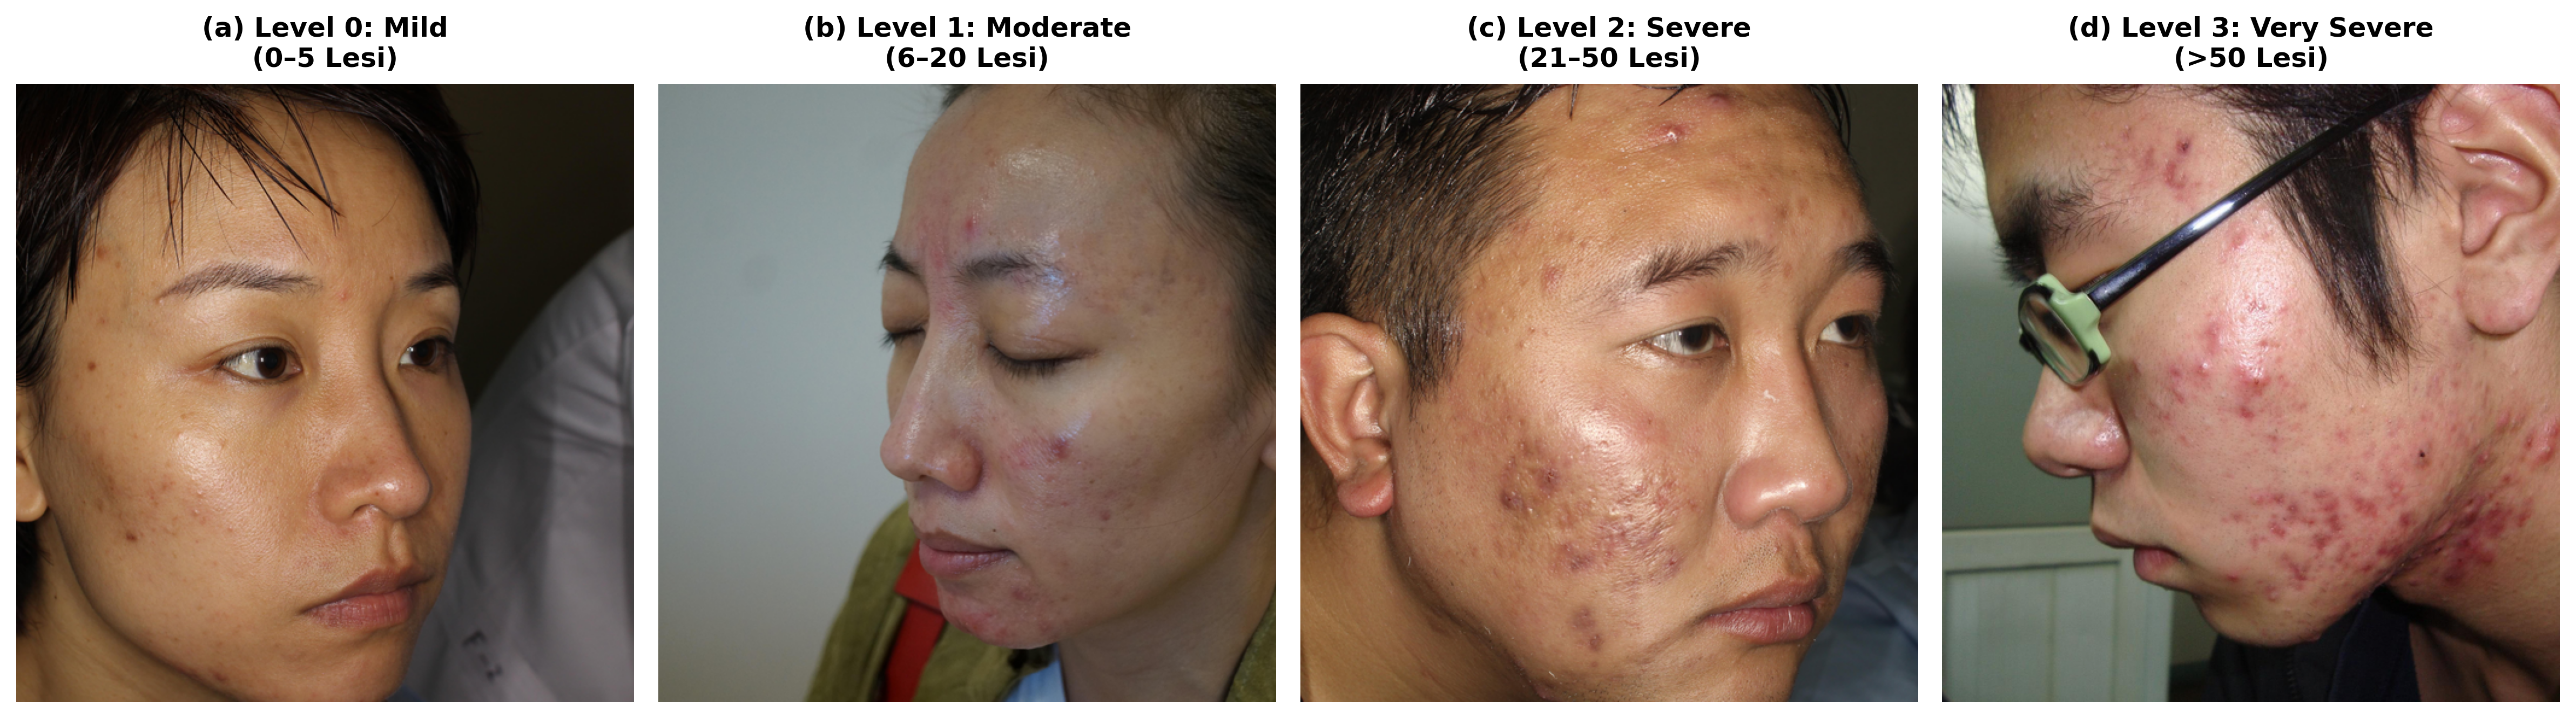
\includegraphics[width=\textwidth]{Gambar/acne04_collage_1x4_id.png}
    \caption{Sampel Citra Representatif Keempat Kelas Keparahan Jerawat (Level 0--3) pada Dataset \texttt{Layered-Labs/ACNE04} Berdasarkan Kriteria Hayashi.}
    \label{fig:acne04_collage}
\end{figure}

\subsection{\textit{Exploratory Data Analysis} (EDA)}
\label{subsec:eda_acne04}

Untuk memperoleh pemahaman empiris mengenai karakteristik fisik, struktur statistik, dan variabilitas visual dataset ACNE04 ($N = 1.457$), dilakukan prosedur \textit{Exploratory Data Analysis} (EDA) secara otomatis sebelum perancangan model.

\subsubsection{\textit{Class Distribution} dan \textit{Class Imbalance}}
Hasil audit empiris terhadap dataset \texttt{Layered-Labs/ACNE04} mengonfirmasi adanya \textit{class imbalance} yang substansial antarkelas. Distribusi kuantitatif dan proporsi relatif keempat kelas disajikan pada Gambar~\ref{fig:eda_class_distribution}.

\begin{figure}[!htbp]
    \centering
    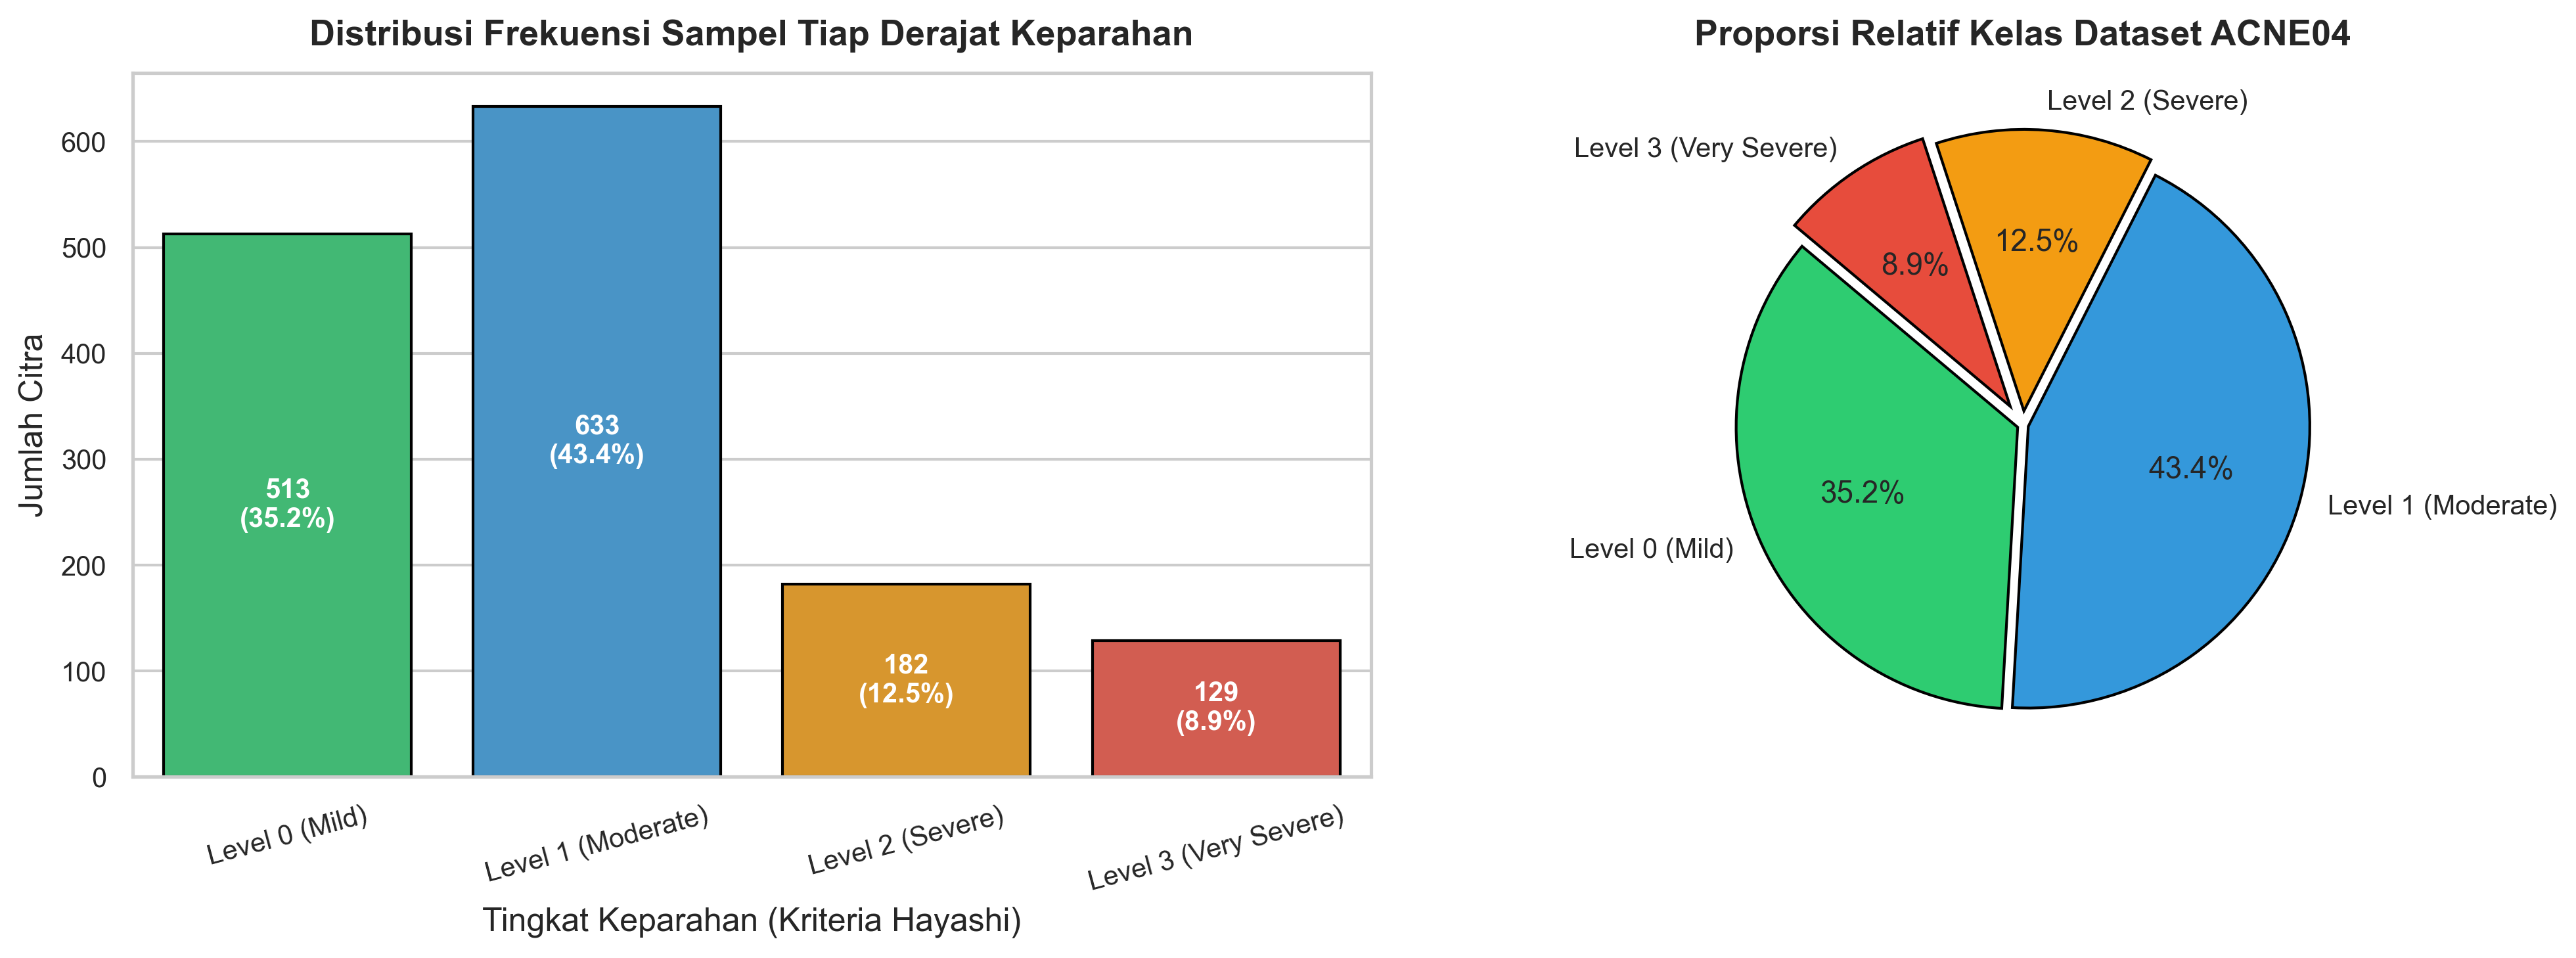
\includegraphics[width=0.92\textwidth]{Gambar/eda_class_distribution.png}
    \caption{Distribusi Frekuensi Sampel dan Proporsi Relatif Kelas pada Dataset ACNE04.}
    \label{fig:eda_class_distribution}
\end{figure}

Berdasarkan Gambar~\ref{fig:eda_class_distribution}, kelas mayoritas terkonsentrasi pada Level 1 (\textit{Moderate}) sebanyak $633$ citra ($43,45\%$) dan Level 0 (\textit{Mild}) sebanyak $513$ citra ($35,21\%$). Sebaliknya, kelas dengan tingkat keparahan tinggi memiliki jumlah sampel jauh lebih sedikit, yaitu Level 2 (\textit{Severe}) sebanyak $182$ citra ($12,49\%$) dan Level 3 (\textit{Very Severe}) sebanyak $129$ citra ($8,85\%$). Rasio \textit{class imbalance} antara kelas terbanyak (Level 1) dan kelas tersedikit (Level 3) mencapai $4,91 : 1,0$. Ketimpangan distribusi ini menjadi tantangan kritis karena fungsi \textit{cross-entropy} standar cenderung bias ke kelas mayoritas dan menurunkan sensitivitas terhadap kasus parah \cite{vut2025, zeng2026}, sehingga mendasari penggunaan \textit{weighted loss} serta metrik \textit{Macro F1-Score}, QWK, dan \textit{Class 3 Recall}.

\subsubsection{Karakteristik Dimensi Spasial dan \textit{File Size}}
Pemeriksaan dimensi geometris terhadap korpus \texttt{Layered-Labs/\allowbreak ACNE04} menunjukkan keberadaan $155$ resolusi spasial unik yang heterogen dengan lebar berkisar antara $143$ hingga $5.184$ piksel (median $3.112$ piksel), tinggi antara $155$ hingga $3.456$ piksel (median $3.456$ piksel), serta rasio aspek berkisar $0,562$--$1,778$ (median $0,900$). Sementara itu, ukuran berkas terkompresi memiliki median $855,49\text{ KB}$ (rentang interkuartil $679,99$--$962,80\text{ KB}$; minimum $3,25\text{ KB}$ dan maksimum $1.353,24\text{ KB}$). Heterogenitas resolusi dan komposisi latar belakang tersebut memvalidasi urgensi tahapan \textit{face cropping} dan standarisasi spasial menjadi $224\times224$ piksel sebelum pemrosesan \textit{Vision Transformer}.

\subsubsection{Profil Eritema (\textit{Erythema Index}) dan \textit{Color Space}}
Manifestasi peradangan jerawat secara visual dicirikan oleh eritema (kemerahan kulit akibat vasodilatasi vaskular). Untuk mengkuantifikasi kromatisitas ini pada sampel berimbang ($100$ citra per kelas), diekstraksi intensitas kanal Merah ($R$) RGB dan kanal $a^*$ dalam \textit{color space} perseptual CIE-LAB (sumbu hijau--merah), sebagaimana ditampilkan pada Gambar~\ref{fig:eda_erythema}.

\begin{figure}[!htbp]
    \centering
    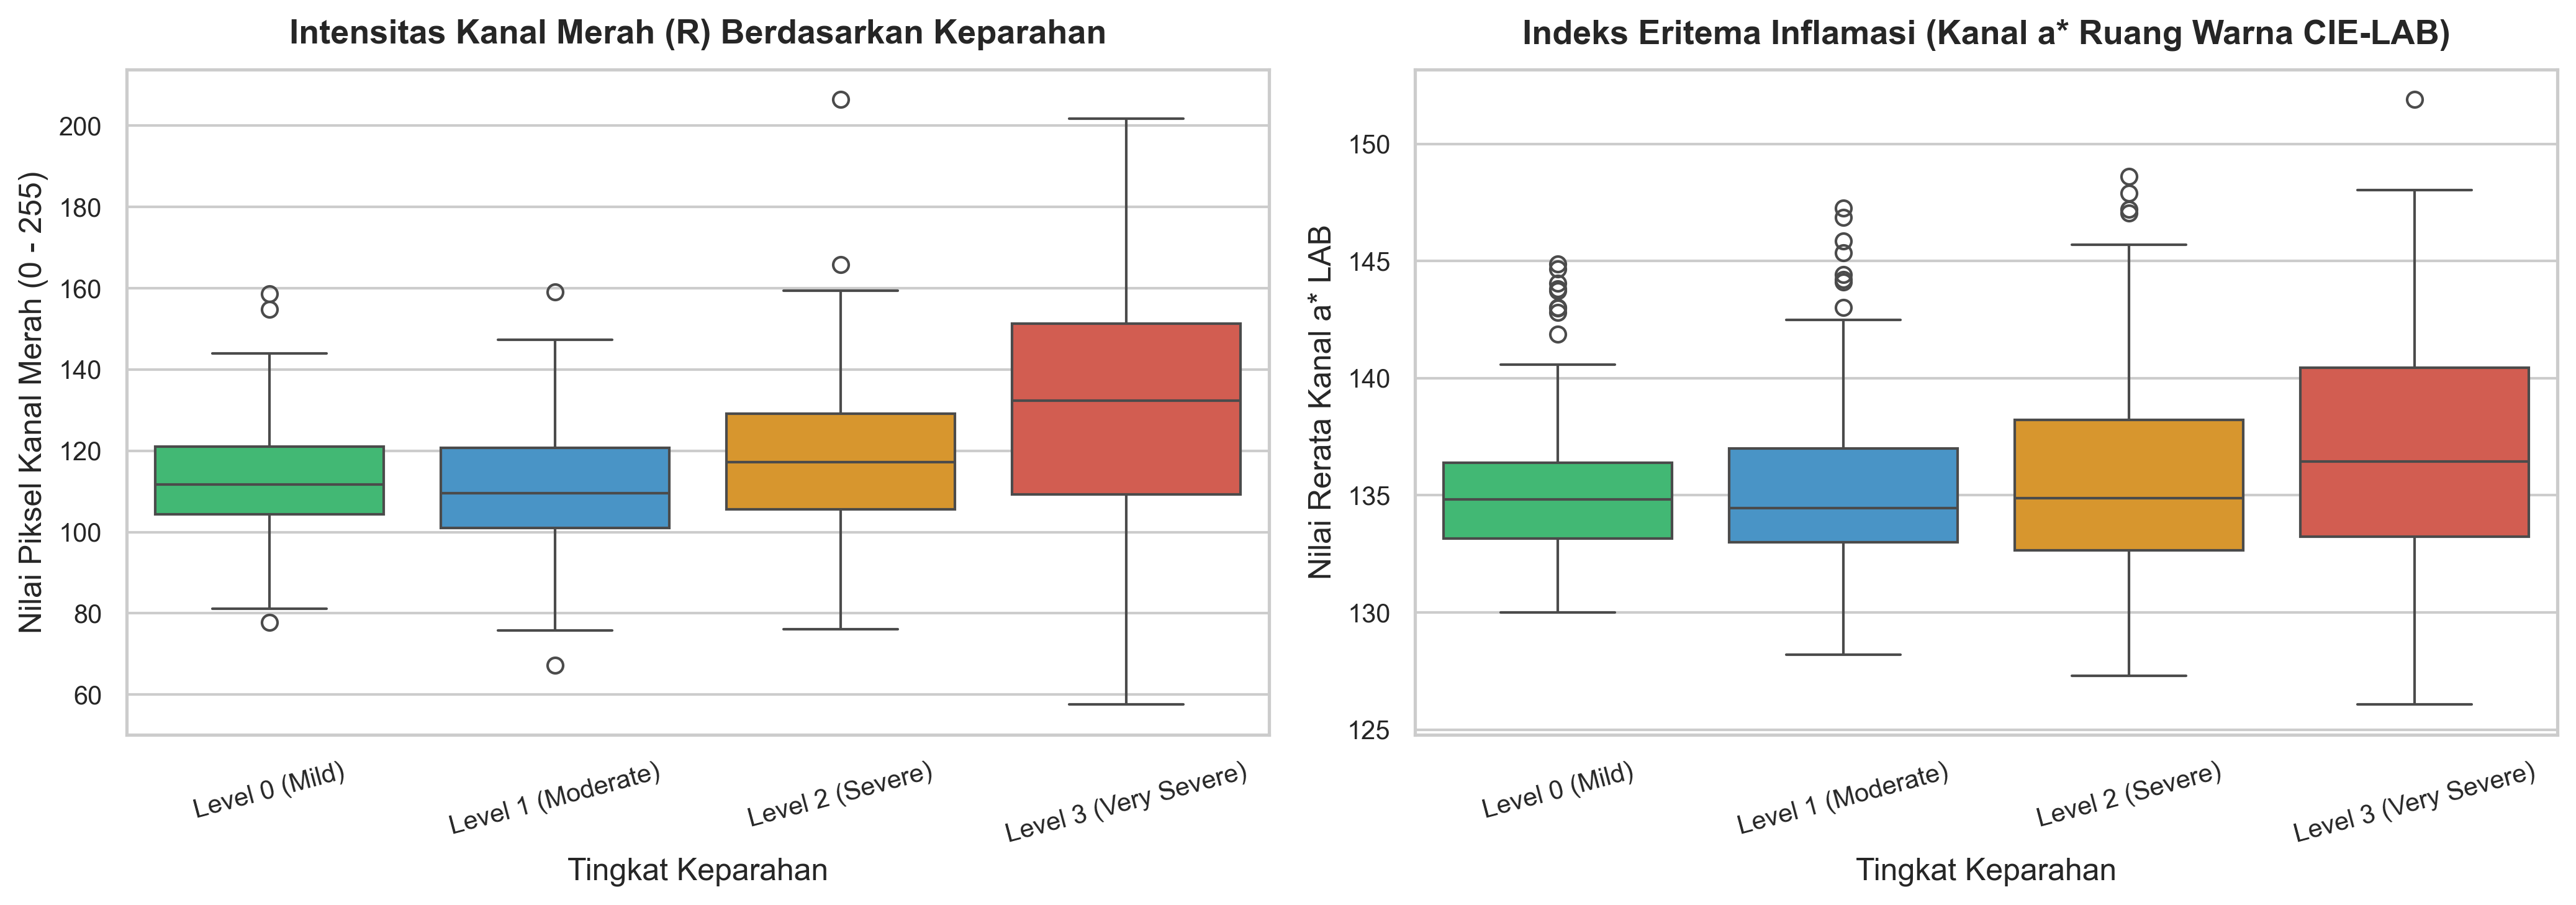
\includegraphics[width=0.92\textwidth]{Gambar/eda_erythema_analysis.png}
    \caption{Profil Distribusi Intensitas Kanal Merah dan Indeks Eritema (Kanal $a^*$ CIE-LAB) Berdasarkan Tingkat Keparahan Jerawat.}
    \label{fig:eda_erythema}
\end{figure}

Gambar~\ref{fig:eda_erythema} memperlihatkan kecenderungan peningkatan indeks kemerahan pada kanal $a^*$ CIE-LAB seiring naiknya tingkat keparahan, yakni dari rerata $135,43$ ($\sigma = 3,20$; median $134,82$) pada Level 0 menuju rerata $137,23$ ($\sigma = 5,53$; median $136,46$) pada Level 3 (\textit{Very Severe}). Tumpang tindih sebaran antar-kelas akibat perbedaan temperatur pencahayaan pemotretan memperkuat alasan penerapan \textit{color constancy} (\textit{Gray World}) serta penajaman kontras lokal (CLAHE).

\subsubsection{Normalisasi Empiris Dataset vs. Konstanta ImageNet}
Perhitungan statistik piksel global di seluruh $1.457$ citra \texttt{Layered-Labs/\allowbreak ACNE04} menghasilkan rerata RGB empiris $\mu = [0,4582;\allowbreak\; 0,3612;\allowbreak\; 0,2935]$ dan standar deviasi $\sigma = [0,2681;\allowbreak\; 0,2134;\allowbreak\; 0,1820]$. Dibandingkan dengan konstanta ImageNet ($\mu = [0,485;\; 0,456;\; 0,406]$ dan $\sigma = [0,229;\; 0,224;\; 0,225]$), terlihat pergeseran intensitas yang dominan ke spektrum \textit{warm skin tones}. Disparitas tersebut menegaskan adanya \textit{domain shift} antara citra objek alamiah dan fotografi dermatologi klinis sehingga menuntut \textit{fine-tuning} bobot DINOv3 secara teratur.

\subsection{\textit{Stratified Data Splitting}}
Untuk mencegah \textit{data leakage} sekaligus mempertahankan komposisi keempat kelas ordinal di setiap subset, $1.457$ citra dibagi menggunakan \textit{stratified split} 70:15:15 dengan perincian sebagai berikut:
\begin{itemize}
    \item \textbf{\textit{Train Set} (70\%):} $1.019$ citra (Level 0: $359$; Level 1: $443$; Level 2: $127$; Level 3: $90$), digunakan untuk pembaruan bobot model.
    \item \textbf{\textit{Validation Set} (15\%):} $219$ citra (Level 0: $77$; Level 1: $95$; Level 2: $27$; Level 3: $20$), digunakan untuk pemantauan \textit{validation loss}, \textit{learning rate scheduler}, dan pemilihan \textit{best checkpoints}.
    \item \textbf{\textit{Test Set} (15\%):} $219$ citra (Level 0: $77$; Level 1: $95$; Level 2: $28$; Level 3: $19$), dijaga terisolasi penuh untuk evaluasi akhir.
\end{itemize}

% -----------------------------------------------------------------------------
\section{\textit{Unified Single-Stream Preprocessing Pipeline}}
\label{sec:pipa_praproses}

Untuk menjamin konsistensi masukan antar-arsitektur pembanding, penelitian ini menerapkan \textit{unified single-stream preprocessing pipeline}. Seluruh citra melewati tahapan pembersihan latar belakang non-kulit, kalibrasi temperatur warna, peningkatan kontras lesi, isolasi area kulit wajah, standarisasi tensor, serta augmentasi klinis khusus \textit{Train Set} sebagaimana dirangkum pada Tabel~\ref{tab:tahap_preprocessing}. Ilustrasi visual perbandingan citra sebelum pemrosesan (\textit{before}), sesudah \textit{preprocessing} deterministik, dan sesudah augmentasi data disajikan pada Gambar~\ref{fig:before_after_preprocessing}.

\begin{table}[!htbp]
    \centering
    \caption{Tahapan \textit{Preprocessing} Satu Jalur dan Penanganan \textit{Class Imbalance}.}
    \label{tab:tahap_preprocessing}
    \footnotesize
    \renewcommand{\arraystretch}{1.25}
    \begin{tabularx}{\textwidth}{c >{\raggedright\arraybackslash}p{3.0cm} >{\raggedright\arraybackslash}X >{\raggedright\arraybackslash}X}
        \toprule
        \textbf{No} & \textbf{Komponen \textit{Pipeline}} & \textbf{Metode Operasional}                                                                                                      & \textbf{Deskripsi}                                                                                                               \\
        \midrule
        1           & \textit{Face Cropping}         & Deteksi wajah otomatis berbasis Haar Cascade dengan \textit{margin padding} 15\%                                         & Mengeliminasi latar belakang non-kulit (rambut, kerah pakaian, dinding) yang berpotensi memicu \textit{spurious features}.       \\
        \midrule
        2           & \textit{Skin Masking}          & Segmentasi area kulit lembut (\textit{soft skin mask}, $\alpha = 0,15$) melalui fusi \textit{color space} HSV dan YCbCr                             & Mereduksi intensitas wilayah non-epidermal sebesar 85\% agar representasi atensi berfokus pada permukaan kulit wajah.            \\
        \midrule
        3           & \textit{Color Constancy}       & Normalisasi \textit{white balance} menggunakan algoritma \textit{Gray World}                                                         & Menetralkan penyimpangan temperatur warna yang disebabkan sensor kamera dan pencahayaan ruangan heterogen.                       \\
        \midrule
        4           & \textit{CLAHE}                 & \textit{Contrast Limited Adaptive Histogram Equalization} ($clip=2,0$, \textit{grid} $8\times8$) pada kanal Luminansi ($L$) CIE-LAB          & Mempertajam visibilitas struktur mikrolesi (komedo, papula, pustula) tanpa merusak rona warna alami kulit.                      \\
        \midrule
        5           & \textit{Resize \& Normalize}   & Penyesuaian resolusi spasial $224\times224$ piksel dan normalisasi tensor RGB                                                    & Menyeragamkan dimensi tensor masukan agar terpartisi presisi menjadi 196 \textit{patches} berukuran $16\times16$ pada \textit{Vision Transformer}. \\
        \midrule
        6           & \textit{Data Augmentation} (\textit{Train Only}) & \textit{Random Horizontal Flip} ($p=0,5$), \textit{Safe Random Rotation} ($\pm15^\circ$), dan \textit{mild ColorJitter} ($\pm10\%$) & Menambah keragaman pose dan pencahayaan wajar tanpa mengubah jumlah maupun karakter patologis lesi kulit.                        \\
        \midrule
        7           & \textit{Cost-Sensitive Weight} & Pembobotan \textit{loss function} \textit{Weighted Cross-Entropy} berbasis frekuensi invers kelas                                & Mengatasi bias mayoritas dan mempertahankan sensitivitas deteksi terhadap kasus minoritas parah (Level 3).                       \\
        \bottomrule
    \end{tabularx}
\end{table}

\begin{figure}[!htbp]
    \centering
    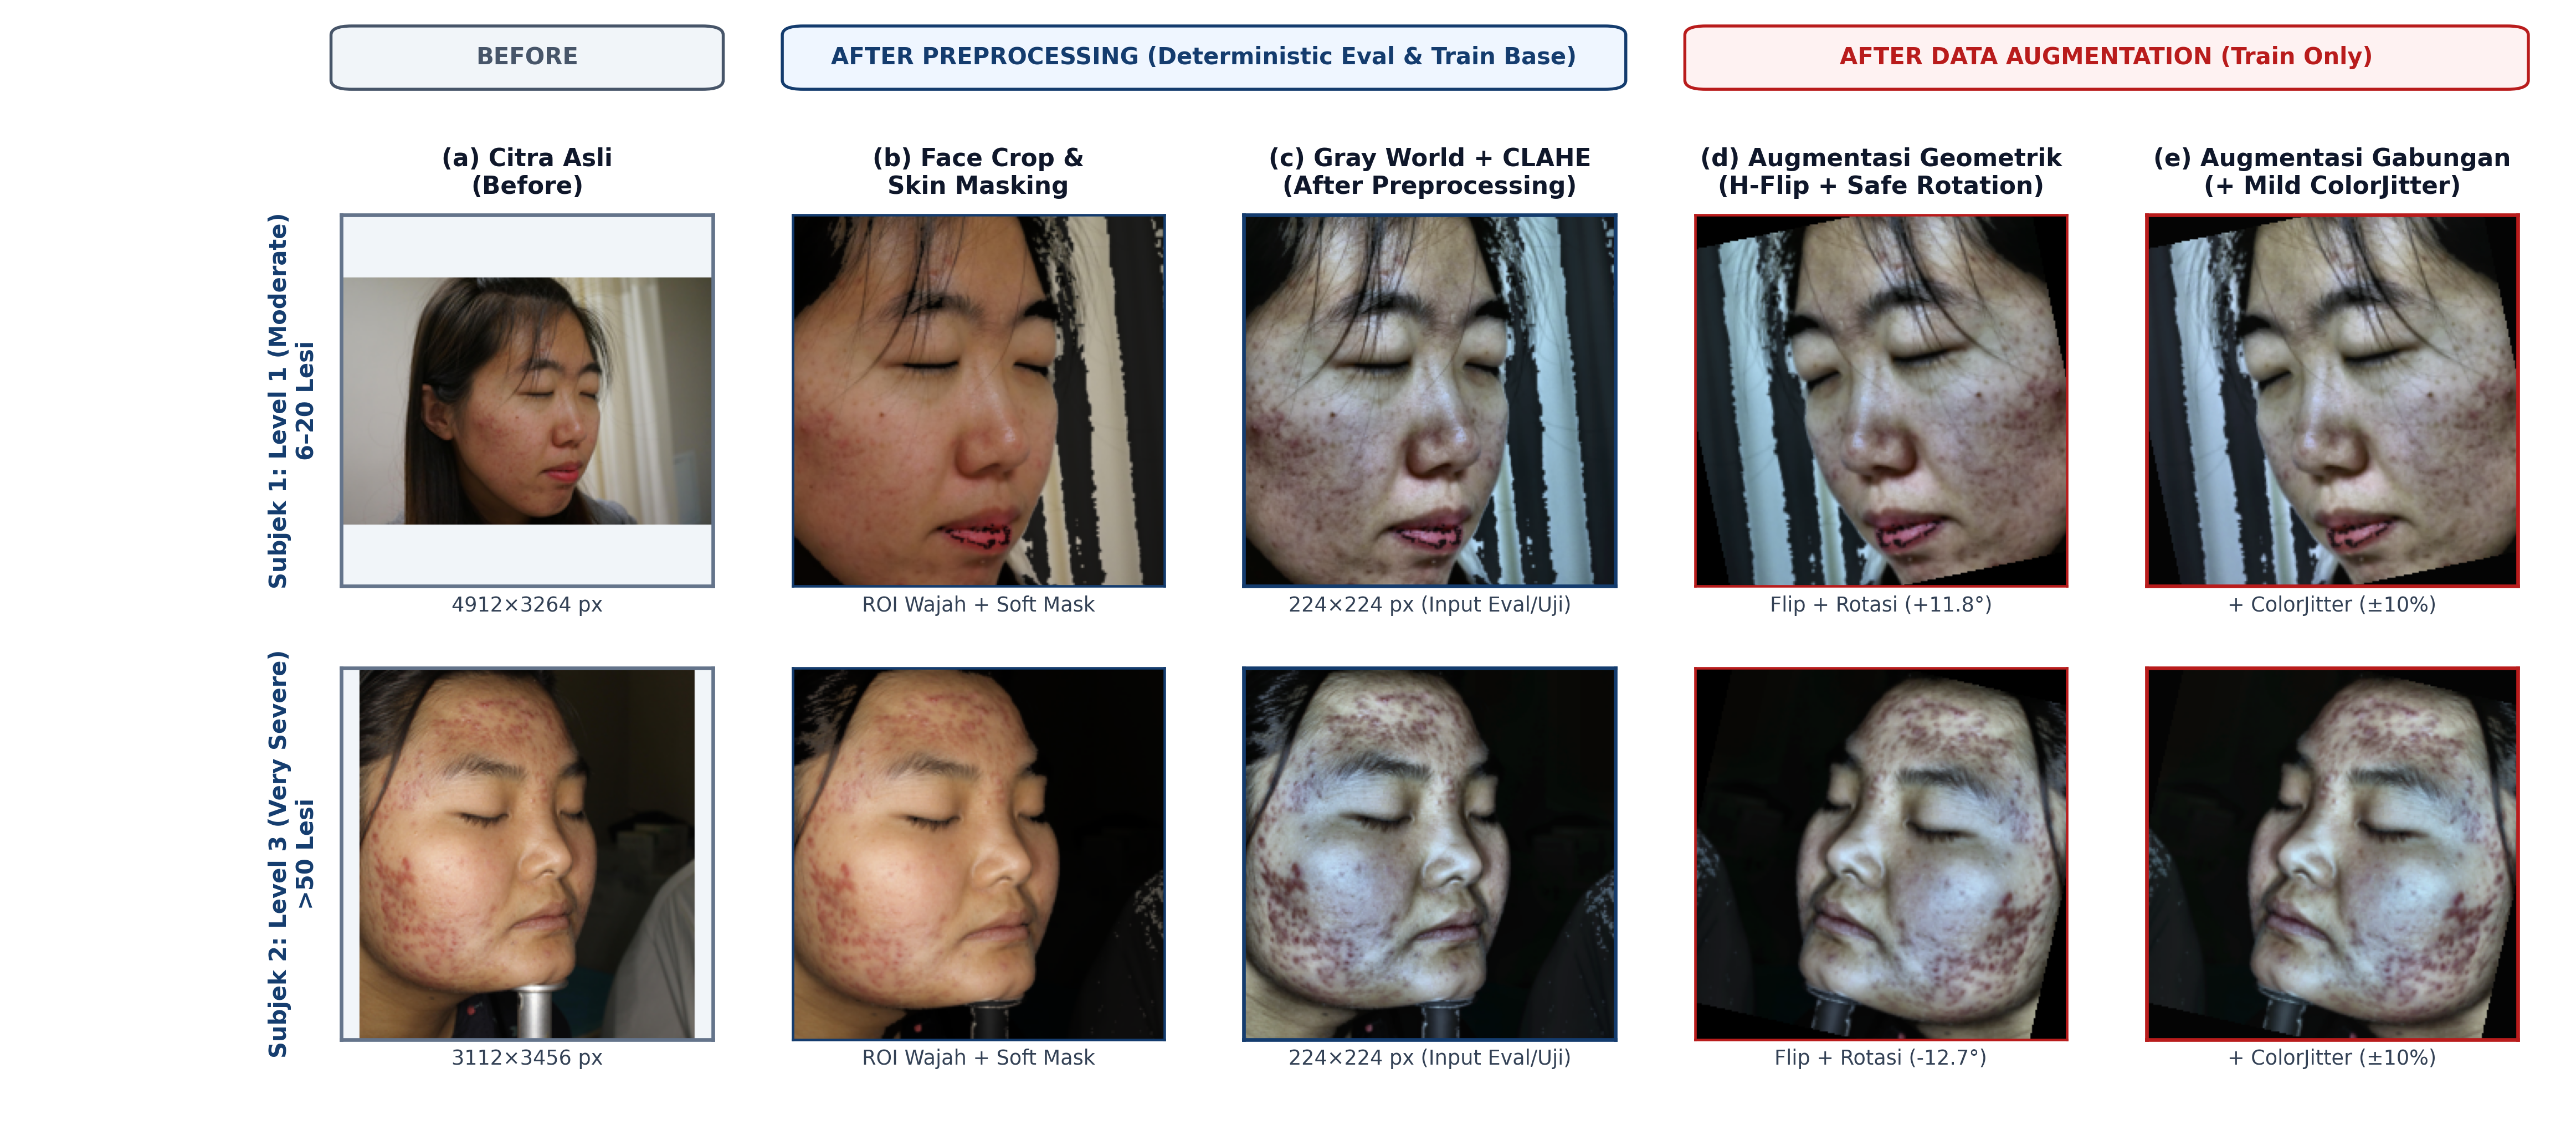
\includegraphics[width=\textwidth]{Gambar/preprocessing_augmentation_before_after.png}
    \caption{Perbandingan Visual Citra Sampel ACNE04 (Level 1 dan Level 3) pada kondisi awal (\textit{Before}), Sesudah \textit{Preprocessing} ($224\times224$ Piksel), dan Sesudah Augmentasi Data Klinis.}
    \label{fig:before_after_preprocessing}
\end{figure}

Secara khusus, pemilihan teknik \textit{data augmentation} hanya diterapkan pada \textit{Train Set} dengan batasan klinis yang masuk akal secara \textit{label-preserving}. Ketiga transformasi augmentasi yang dipilih beserta justifikasinya adalah:
\begin{itemize}
    \item \textbf{\textit{Random Horizontal Flip} ($p=0,5$):} Wajah manusia bersifat simetris secara bilateral; pencerminan horizontal kiri--kanan menyimulasikan variasi sudut pengambilan wajah tanpa mengubah jumlah total maupun klasifikasi tingkat keparahan lesi inflamasi.
    \item \textbf{\textit{Safe Random Rotation} ($\pm 15^\circ$):} Mengakomodasi variasi kemiringan posisi kepala pasien yang realistis saat pemeriksaan foto klinis. Sebaliknya, rotasi ekstrem maupun \textit{vertical flip} dihindari karena tidak realistis secara anatomis.
    \item \textbf{\textit{Mild ColorJitter} (\textit{brightness}, \textit{contrast}, \textit{saturation} $\pm 0,10$; \textit{hue} $\pm 0,03$):} Memperkaya variasi kecerahan dan kontras ruangan secara terukur; pergeseran \textit{hue} dibatasi ketat maksimal $\pm 0,03$ agar tidak mengubah eritema kemerahan secara artifisial. Transformasi destruktif seperti \textit{random erasing/cutout} juga dihindari karena berisiko menutupi kelompok pustula dan mengubah kelas label.
\end{itemize}

\subsection{Formulasi Matematis \textit{Preprocessing} dan \textit{Loss Weighting}}

\subsubsection{\textit{Contrast Limited Adaptive Histogram Equalization} (CLAHE)}
CLAHE diterapkan pada kanal luminansi ($L$) dari \textit{color space} CIE-LAB untuk mencegah amplifikasi \textit{noise} pada area homogen kulit \cite{wang2023}. Citra dibagi menjadi kisi blok kontekstual berukuran $8\times8$ piksel dengan pembatasan kontras (\textit{clipping limit} $= 2,0$), lalu kelebihan piksel didistribusikan merata sebelum interpolasi bilinear.

\subsubsection{\textit{Color Constancy} (\textit{Gray World})}
Variasi temperatur warna dinetralkan menggunakan algoritma \textit{Gray World}, yang mengasumsikan rerata reflektansi ketiga kanal warna mencerminkan abu-abu netral:
\begin{equation}
    k_c = \frac{1}{|I|} \sum_{x,y} I_c(x,y), \quad c \in \{R, G, B\}
\end{equation}
Setiap kanal diskalakan terhadap rata-rata global $\mu = \frac{k_R + k_G + k_B}{3}$ sehingga $I'_c(x,y) = I_c(x,y) \times \frac{\mu}{k_c}$.

\subsubsection{\textit{Cost-Sensitive Loss Weighting}}
Untuk mengompensasi rasio ketimpangan $4,91 : 1,0$, diterapkan bobot penalti frekuensi invers pada \textit{loss function} untuk setiap kelas $c \in \{0, 1, 2, 3\}$:
\begin{equation}
    w_c = \frac{N_{\text{train}}}{K \cdot N_c}
\end{equation}
dengan $N_{\text{train}} = 1.019$ adalah jumlah total sampel \textit{Train Set}, $K = 4$ jumlah kelas, dan $N_c$ jumlah sampel kelas $c$. Dengan formulasi ini, kelas minoritas Level 3 (\textit{Very Severe}, $N_3 = 90$) memperoleh bobot penalti tertinggi sehingga kesalahan prediksi pada kelas parah ditekan lebih kuat selama \textit{backpropagation}.

% -----------------------------------------------------------------------------
\section{Desain Arsitektur Model \textit{Transfer Learning}}
\label{sec:perancangan_arsitektur}

Penelitian ini mengadaptasi serta membandingkan dua skala arsitektur \textit{Vision Transformer} (ViT) dari keluarga \textit{vision foundation model} \textit{self-supervised} DINOv3 \cite{simeoni2025dinov3}. Rincian topologi blok encoder, \textit{register tokens}, dan perbandingan spesifikasi keduanya telah dipaparkan secara utuh pada Gambar~\ref{fig:arsitektur_dinov3} dan Tabel~\ref{tab:spesifikasi_dinov3} di Bab~II, yakni \textbf{DINOv3 ViT-L/16} (\textit{heavyweight}: 24 blok, $d=1.024$, 16 \textit{attention heads}, $\approx 304\text{M}$ parameter) serta \textbf{DINOv3 ViT-S/16} (\textit{lightweight}: 12 blok, $d=384$, 6 \textit{attention heads}, $\approx 21,6\text{M}$ parameter).

\subsection{\textit{Architecture Flow} dan \textit{Classification Head}}
Kedua model diinisialisasi menggunakan \textit{pre-trained weights} resmi DINOv3 \cite{simeoni2025dinov3} dan mengikuti aliran arsitektur terpadu dari tahap tokenisasi hingga klasifikasi ordinal. Citra wajah ter-preprocess berdimensi $224 \times 224 \times 3$ terlebih dahulu melalui lapisan konvolusi \textit{patch embedding} berukuran $16 \times 16$ piksel (\textit{stride} 16), menghasilkan kisi $14 \times 14 = 196$ \textit{patch tokens} yang digabungkan bersama satu token global \texttt{[CLS]}, empat \textit{register tokens}, serta \textit{axial Rotary Position Embedding} (RoPE). Rangkaian token tersebut melewati $L$ blok \textit{Transformer Encoder} ($L=24$ untuk ViT-L/16; $L=12$ untuk ViT-S/16) guna memodelkan relasi spasial lintas-area wajah. Pada luaran blok terakhir, vektor representasi token global \texttt{[CLS]} diekstraksi sebagai ringkasan fitur wajah menyeluruh:
\begin{equation}
    \mathbf{v}_{\text{[CLS]}} \in \mathbb{R}^{d_{\text{in}}}
\end{equation}
di mana $d_{\text{in}} = 1.024$ untuk DINOv3 ViT-L/16 dan $d_{\text{in}} = 384$ untuk DINOv3 ViT-S/16.

Untuk memetakan vektor laten ke empat kelas keparahan jerawat ordinal (Level 0--3), dibangun lapisan \textit{Linear Classification Head} kustom dengan regularisasi \textit{Dropout}:
\begin{equation}
    \mathbf{v}_{\text{[CLS]}} \xrightarrow{\text{Dropout}(p=0,2)} \mathbf{v}' \xrightarrow{\text{Linear}(d_{\text{in}} \to 4)} \hat{\mathbf{z}} \in \mathbb{R}^4
\end{equation}
Vektor \textit{logits} $\hat{\mathbf{z}}$ kemudian dikonversi melalui fungsi aktivasi \textit{softmax} menjadi distribusi probabilitas empat kelas:
\begin{equation}
    \hat{y}_c = \frac{\exp(\hat{z}_c)}{\sum_{j=0}^{3} \exp(\hat{z}_j)}, \quad c \in \{0, 1, 2, 3\}
\end{equation}

% -----------------------------------------------------------------------------
\section{Skenario \textit{Training} dan Optimasi}
\label{sec:skenario_pelatihan}

Proses \textit{training} seluruh model dijalankan menggunakan protokol komputasi dan lingkungan terstandarisasi berbasis pustaka PyTorch. Konfigurasi \textit{hyperparameter} eksperimen dirangkum pada Tabel~\ref{tab:hiperparameter_pelatihan}.

\begin{table}[!htbp]
    \centering
    \caption{Konfigurasi \textit{Hyperparameter Training} Model \textit{Transfer Learning} DINOv3.}
    \label{tab:hiperparameter_pelatihan}
    \small
    \renewcommand{\arraystretch}{1.25}
    \begin{tabularx}{\textwidth}{l >{\raggedright\arraybackslash}X}
        \toprule
        \textbf{\textit{Hyperparameter}}               & \textbf{Nilai / Konfigurasi}                                                             \\
        \midrule
        Arsitektur Model                               & DINOv3 ViT-L/16 (\textit{Heavyweight}) dan DINOv3 ViT-S/16 (\textit{Lightweight})        \\
        \textit{Input Dimension}                       & $224 \times 224 \times 3$ piksel ($196$ \textit{patch tokens} berukuran $16\times16$)     \\
        \textit{Batch Size}                            & $16$                                                                                     \\
        \textit{Optimizer}                             & AdamW (\textit{weight decay} $= 1\times 10^{-4}$)                                        \\
        \textit{Initial Learning Rate} ($\eta_0$)      & $1\times 10^{-4}$ (ViT-S/16) dan $5\times 10^{-5}$ (ViT-L/16)                            \\
        \textit{Learning Rate Scheduler}               & \textit{Cosine Annealing} ($T_{\text{max}} = 50$, $\eta_{\text{min}} = 1\times 10^{-6}$) \\
        \textit{Loss Function}                         & \textit{Weighted Categorical Cross-Entropy Loss}                                         \\
        Maksimum \textit{Epoch}                        & $50$ \textit{epoch}                                                                      \\
        \textit{Early Stopping}                        & \textit{Patience} $= 10$ \textit{epoch} pada metrik \textit{Validation Macro-F1}         \\
        Perangkat Keras                                & NVIDIA GPU dengan akselerasi CUDA                                                        \\
        \bottomrule
    \end{tabularx}
\end{table}

\subsection{\textit{Input Dimension} dan \textit{Batch Size}}
Dimensi spasial citra masukan ditetapkan sebesar $224 \times 224 \times 3$ piksel sehingga citra terpartisi presisi menjadi kisi $14 \times 14$ ($196$ \textit{patch tokens}) berukuran $16 \times 16$ piksel tanpa distorsi interpolasi. Resolusi ini menjaga ketajaman tekstur mikrolesi jerawat sekaligus menstabilkan kebutuhan memori VRAM GPU \cite{simeoni2025dinov3}.

Nilai \textit{batch size} ditetapkan sebesar $16$ sampel per iterasi guna mengakomodasi graf komputasi DINOv3 ViT-L/16 ($\approx 304\text{M}$ parameter) pada satu GPU serta memberikan regularisasi gradien stokastik pada \textit{Train Set} ($N_{\text{train}} = 1.019$) \cite{davila2024}.

\subsection{\textit{Optimizer} dan \textit{Weight Decay}}
Optimasi parameter menggunakan \textit{optimizer} AdamW (\textit{decoupled weight decay}) dengan koefisien \textit{weight decay} $= 1 \times 10^{-4}$. Pada arsitektur \textit{Vision Transformer}, pemisahan \textit{weight decay} dari estimasi momen adaptif mencegah distorsi skala gradien sehingga meminimalkan risiko \textit{catastrophic forgetting} terhadap representasi umum \textit{vision foundation model} DINOv3 \cite{simeoni2025dinov3}.

\subsection{\textit{Learning Rate} dan \textit{Cosine Annealing Scheduler}}
Nilai \textit{initial learning rate} ditetapkan $\eta_0 = 1 \times 10^{-4}$ untuk DINOv3 ViT-S/16 dan $\eta_0 = 5 \times 10^{-5}$ yang lebih konservatif untuk DINOv3 ViT-L/16 agar pembaruan bobot pada $24$ blok atensi tidak memicu osilasi gradien awal. Peluruhan \textit{learning rate} selama $50$ \textit{epoch} dikendalikan melalui \textit{Cosine Annealing Scheduler}:
\begin{equation}
    \eta_t = \eta_{\text{min}} + \frac{1}{2}(\eta_0 - \eta_{\text{min}})\left(1 + \cos\left(\frac{t}{T_{\text{max}}}\pi\right)\right)
\end{equation}
dengan $\eta_{\text{min}} = 1 \times 10^{-6}$ dan $T_{\text{max}} = 50$.

\subsection{\textit{Weighted Categorical Cross-Entropy Loss}}
Kondisi \textit{class imbalance} dataset \texttt{Layered-Labs/ACNE04} (rasio Level 1 terhadap Level 3 sebesar $4,91 : 1,0$) dimitigasi menggunakan \textit{loss function} \textit{Weighted Categorical Cross-Entropy} ($\mathcal{L}_{\text{WCE}}$):
\begin{equation}
    \mathcal{L}_{\text{WCE}} = - \frac{1}{B} \sum_{i=1}^{B} \sum_{c=0}^{3} w_c \cdot y_{i,c} \log(\hat{y}_{i,c})
\end{equation}
di mana $B = 16$ adalah \textit{batch size}, $y_{i,c} \in \{0, 1\}$ label \textit{one-hot}, $\hat{y}_{i,c}$ probabilitas \textit{softmax}, dan $w_c = \frac{N_{\text{train}}}{K \cdot N_c}$ bobot penalti kelas ($N_{\text{train}} = 1.019$, $K = 4$). Kesalahan klasifikasi pada kelas minoritas Level 3 dikenakan penalti gradien terbesar agar model membentuk batas keputusan yang seimbang di seluruh kelas \cite{vut2025}.

\subsection{\textit{Convergence Criteria} dan \textit{Early Stopping}}
Proses \textit{training} dijalankan hingga maksimum $50$ \textit{epoch} dengan mekanisme \textit{early stopping} (\textit{patience} $= 10$ \textit{epoch}) yang memantau \textit{Validation Macro-F1} guna mencegah \textit{overfitting}. Bobot model terbaik (\textit{best checkpoint}) dipilih untuk evaluasi akhir.

% -----------------------------------------------------------------------------
\section{Metrik Evaluasi Kinerja}
\label{sec:metrik_evaluasi}

Kinerja seluruh model diuji secara menyeluruh pada subset \textit{Test Set} independen yang terisolasi ($N_{\text{test}} = 219$; distribusi: Level 0 $= 77$, Level 1 $= 95$, Level 2 $= 28$, Level 3 $= 19$). Mengingat ketimpangan distribusi serta sifat ordinal tingkat keparahan jerawat, evaluasi mengombinasikan akurasi global, metrik \textit{macro-averaging}, kesepakatan ordinal \textit{Quadratic Weighted Kappa}, sensitivitas Level 3, dan \textit{confusion matrix} numerik \cite{davila2024, vut2025}.

\subsection{\textit{Accuracy}}
\textit{Accuracy} mengukur proporsi total prediksi tepat terhadap seluruh sampel uji ($N_{\text{test}} = 219$):
\begin{equation}
    \text{Accuracy} = \frac{\sum_{c=0}^{3} TP_c}{N_{\text{test}}}
\end{equation}
dengan $TP_c$ menyatakan jumlah \textit{True Positive} kelas ke-$c$.

\subsection{\textit{Macro Precision}}
\textit{Macro Precision} mengevaluasi ketepatan rata-rata prediksi positif secara merata di seluruh empat kelas (Level 0, Level 1, Level 2, dan Level 3):
\begin{equation}
    \text{Precision}_{\text{macro}} = \frac{1}{4} \sum_{c=0}^{3} \frac{TP_c}{TP_c + FP_c}
\end{equation}
di mana $FP_c$ adalah jumlah \textit{False Positive} kelas ke-$c$. Presisi yang tinggi pada seluruh kelas meminimalkan risiko \textit{over-diagnosis} yang dapat berujung pada intervensi klinis berlebih \cite{hayashi2008, lopez2023}.

\subsection{\textit{Macro Recall}}
\textit{Macro Recall} mengukur rata-rata kemampuan model menjaring kembali seluruh sampel aktual pada keempat kelas (Level 0, Level 1, Level 2, dan Level 3):
\begin{equation}
    \text{Recall}_{\text{macro}} = \frac{1}{4} \sum_{c=0}^{3} \frac{TP_c}{TP_c + FN_c}
\end{equation}
di mana $FN_c$ adalah jumlah \textit{False Negative} kelas ke-$c$, yang mencerminkan kemampuan pencegahan \textit{under-diagnosis} secara merata di seluruh kelas tanpa didominasi kelas mayoritas.

\subsection{\textit{Macro F1-Score}}
\textit{Macro F1-Score} menghitung rata-rata harmonik dari \textit{Precision} dan \textit{Recall} secara setara di seluruh empat kelas:
\begin{equation}
    \text{F1}_{\text{macro}} = \frac{1}{4}\sum_{c=0}^{3} \frac{2 \cdot \text{Precision}_c \cdot \text{Recall}_c}{\text{Precision}_c + \text{Recall}_c}
\end{equation}
Metrik ini dijadikan tolok ukur pemilih model terbaik karena memberi bobot identik $25\%$ pada setiap kelas \cite{davila2024, zeng2026}.

\subsection{\textit{Quadratic Weighted Kappa} (QWK)}
Karena kelas Level 0 hingga Level 3 bersifat ordinal berurutan, kesalahan klasifikasi sejauh tiga tingkat (misalnya Level 3 diprediksi sebagai Level 0) jauh lebih berbahaya secara klinis daripada pergeseran satu tingkat bertetangga. Oleh karena itu, digunakan \textit{Quadratic Weighted Kappa} (QWK, $\kappa_w$) yang mengukur tingkat kesesuaian prediksi terhadap label klinis dengan bobot penalti kuadratik atas jarak kesalahan kelas \cite{cohen1968weighted}:
\begin{equation}
    \kappa_w = 1 - \frac{\sum_{i=0}^{3}\sum_{j=0}^{3} w_{i,j}\, O_{i,j}}{\sum_{i=0}^{3}\sum_{j=0}^{3} w_{i,j}\, E_{i,j}}, \qquad w_{i,j} = \frac{(i - j)^2}{(K - 1)^2}
\end{equation}
di mana $K = 4$, $O_{i,j}$ adalah \textit{confusion matrix} pengamatan, $E_{i,j}$ matriks harapan peluang acak di bawah independensi marginal, dan $w_{i,j} \in [0, 1]$ bobot kuadratik ($w_{0,0}=0$, pergeseran $1$ tingkat $w_{i,i\pm1}=1/9$, sedangkan kesalahan ekstrem $w_{0,3}=1$). Nilai QWK berada pada rentang $[-1, 1]$: nilai $\le 0$ menandakan kesepakatan setara atau lebih buruk dari tebakan acak; nilai $0,01$--$0,40$ dinilai lemah--cukup; $0,41$--$0,60$ sedang (\textit{moderate}), $0,61$--$0,80$ substansial (\textit{substantial}), dan rentang $0,81$--$1,00$ dikategorikan hampir sempurna (\textit{almost perfect agreement}) dan layak untuk sistem penunjang diagnosis klinis \cite{landis1977measurement, zeng2026}.

\subsection{\textit{Class 3 Recall} dan \textit{Confusion Matrix}}
Kesalahan \textit{under-diagnosis} pada pasien Level 3 membawa konsekuensi klinis paling berat karena menunda terapi sistemik \cite{hayashi2008, vut2025}, sehingga sensitivitas kelas paling parah diukur secara khusus melalui:
\begin{equation}
    \text{Recall}_{3} = \frac{C_{3,3}}{\sum_{j=0}^{3} C_{3,j}}
\end{equation}
di mana $C_{i,j}$ merupakan sel pada \textit{confusion matrix} berukuran $4 \times 4$. Sesuai standar penomoran kelas pada Tabel~\ref{tab:distribusi_acne04}, seluruh label baris dan kolom pada \textit{confusion matrix} menggunakan notasi numerik murni (\texttt{0}, \texttt{1}, \texttt{2}, \texttt{3}) guna meringkas tampilan tanpa pengulangan teks kategori (0 = \textit{Mild}, 1 = \textit{Moderate}, 2 = \textit{Severe}, 3 = \textit{Very Severe}), sebagaimana diformat pada Tabel~\ref{tab:template_confusion_matrix}. Selain metrik kuantitatif penuh tersebut, kasus dengan selisih probabilitas top-1 dan top-2 yang sempit ($\Delta p < 0,15$) dicatat sebagai penanda \textit{borderline ambiguity} pada berkas log CSV untuk analisis galat kualitatif di sekitar batas kelas Hayashi.

\begin{table}[!htbp]
    \centering
    \caption{Struktur \textit{Confusion Matrix} Empat Kelas Bernotasi Numerik (\textit{Test Set}, $N_{\text{test}} = 219$).}
    \label{tab:template_confusion_matrix}
    \small
    \renewcommand{\arraystretch}{1.25}
    \begin{tabular}{c c cccc c}
        \toprule
        & & \multicolumn{4}{c}{\textbf{Prediksi Model (\textit{Predicted})}} & \\
        \cmidrule(lr){3-6}
        & & \textbf{0} & \textbf{1} & \textbf{2} & \textbf{3} & \textbf{Total} \\
        \midrule
        \multirow{4}{*}{\makecell{\textbf{Aktual}\\\textbf{(\textit{True})}}}
        & \textbf{0} & $C_{0,0}$ & $C_{0,1}$ & $C_{0,2}$ & $C_{0,3}$ & $77$ \\
        & \textbf{1} & $C_{1,0}$ & $C_{1,1}$ & $C_{1,2}$ & $C_{1,3}$ & $95$ \\
        & \textbf{2} & $C_{2,0}$ & $C_{2,1}$ & $C_{2,2}$ & $C_{2,3}$ & $28$ \\
        & \textbf{3} & $C_{3,0}$ & $C_{3,1}$ & $C_{3,2}$ & $C_{3,3}$ & $19$ \\
        \midrule
        \multicolumn{2}{c}{\textbf{Total}} & $\sum_i C_{i,0}$ & $\sum_i C_{i,1}$ & $\sum_i C_{i,2}$ & $\sum_i C_{i,3}$ & $\mathbf{219}$ \\
        \bottomrule
    \end{tabular}
\end{table}

%

%%%%%%%%%%%%%%%%%%%%%%%%%%%%%%%%%%%%%%%%%%%%%%%%%%%%%%%%%%%%%%%
% Berikut adalah untuk membuat Daftar pustaka
% Style daftar pustaka dapat disesuaikan dengan mengubah 
%\bibliographystyle{kode}
% dengan kode = acm maka hasinya contoh [1]
% dengan kode = agsm maka hasilnya Harvard style (Sukimin, 2017)
%%%%%%%%%%%%%%%%%%%%%%%%%%%%%%%%%%%%%%%%%%%%%%%%%%%%%%%%%%%%%%%%
\cleardoublepage
\addcontentsline{toc}{chapter}{Daftar Pustaka}
\bibliographystyle{plain} %harvard style
\bibliography{References}
%
%\pagebreak
%%%%%%%%%%%%%%%%%%%%%%%%%%%%%%%%%%%%%%%%%%%%%%%%%%%%%%%%%%%%%%%
% Berikut untuk lampiran
%%%%%%%%%%%%%%%%%%%%%%%%%%%%%%%%%%%%%%%%%%%%%%%%%%%%%%%%%%%%%%
\cleardoublepage
\addcontentsline{toc}{chapter}{Lampiran}
% !TEX root = main.tex
\chapter*{Lampiran}

\end{document}
